\documentclass[12pt,letterpaper]{book}
\usepackage[spanish, es-tabla]{babel}
\usepackage[utf8]{inputenc}
\usepackage[colorlinks=true, linkcolor=ginda]{hyperref}
\usepackage{booktabs}
\usepackage{amsmath}
\usepackage{graphicx}
\usepackage{amsfonts}
\usepackage{amssymb}
\usepackage{pdfpages}
\usepackage{makeidx}
\usepackage{import}
\usepackage{listings}
\usepackage{float} 
\usepackage{color}
\usepackage{multirow}
\usepackage{amsfonts}
\usepackage{minitoc}
\usepackage{enumitem}
\usepackage{setspace}
%\usepackage{apacite}
%\usepackage{natbib}
\usepackage[titletoc]{appendix}
%\usepackage{algorithm,algpseudocode}
\usepackage[ruled,vlined]{algorithm2e}
%\usepackage{algorithmicx}
\usepackage[Lenny]{fncychap}
\usepackage{subfigure}
\mtcsettitle{minitoc}{Sumario}
\mtcsetrules{*}{off}
\DeclareMathOperator*{\argmax}{arg\,max}
\DeclareMathOperator*{\argmin}{argmin}
\newcommand{\JSP}{\textbf{JSP}}
\newcommand{\EA}{{\sc ae}}
\newcommand{\DE}{{\sc ed}}
\newcommand{\TS}{{\sc bt}}
\newcommand{\MA}{{\sc am}}
\newcommand{\GCP}{{\sc gcp}}
\newcommand{\KGCP}{k-{\sc gcp}}
\newcommand{\EAS}{{\sc ae}s}
\newcommand{\BNP}{{\sc bnp}}
\newcommand{\CEC}{{\sc cec}}
\newcommand{\PSO}{{\sc pso}}
\newcommand{\BFS}{{\sc bfs}}
\newcommand{\NSGA}{{\sc nsga-ii}}
\newcommand{\DECD}{{\sc decd}}
\newcommand{\BNPC}{{\sc bnpc}}
\newcommand{\OCR}{{\sc ocr}}
\newcommand{\DMACOL}{{\sc dmacol}}
\newcommand{\IEEE}{{\sc ieee}}
\newcommand{\DIMACS}{{\sc dimacs}}
\newcommand{\GECCO} {{\sc gecco}}
\newcommand{\TSP} {{\sc tsp}}
\newcommand{\GPP} {{\sc gpp}}

\newcommand{\SADE}{{\sc sade}}
\newcommand{\SHADE}{{\sc shade}}
\newcommand{\LSHADE}{{\sc l-shade}}
\newcommand{\LSHADECC}{{\sc l-shade44}}
\newcommand{\LSHADEE}{{\sc l-shade44-iepsilon}}
\newcommand{\LSHADEI}{{\sc l-shade44-ide}}
\newcommand{\CODE}{{\sc code}}
\newcommand{\CCODE}{{\sc c$^2$ode}}
\newcommand{\JADE}{{\sc jade}}
\newcommand{\UDE}{{\sc ude}}
\newcommand{\IUDE}{{\sc iude}}
\newcommand{\MAES}{{\sc ma-es}}

\newcommand{\COP}{{\sc cop}s}
\newcommand{\CO}{{\sc co}}
\newcommand{\DEP}{{\sc dep}}
\newcommand{\DEI}{{\sc de}}
\newcommand{\EAI}{{\sc ea}}
\newcommand{\EASI}{{\sc ea}s}

\newcommand{\DEBNP}{{\sc debnp}}
\newcommand{\DSATUR}{{\sc dsatur}}
\newcommand{\GPX}{{\sc gpx}}
\newcommand{\TABUCOL}{{\sc tabucol}}
\newcommand{\HBFSX}{{\sc hbfsx}}
\newcommand{\MBA}{{\sc mba}}
\newcommand{\FAP}{{\sc fap}}

\newcommand{\subsubsubsection}[1]{\paragraph{#1}\mbox{}\\}
\setcounter{secnumdepth}{2}
\setcounter{tocdepth}{2}

\newcommand{\R}{\mathbb{R}}
%\newcommand\tab[1][1cm]{\hspace*{#1}}

%\algdef{SE}[DOWHILE]{Do}{doWhile}{\algorithmicdo}[1]{\algorithmicwhile\ #1}%
%\algrenewcommand\algorithmicprocedure{\textbf{procedimiento}}
%
%\algrenewcommand\algorithmicrequire{\textbf{Entrada:}}
%\algrenewcommand\algorithmicensure{\textbf{Salida:}}
%\algrenewcommand\algorithmicend{\textbf{fin}}
%\algrenewcommand\algorithmicif{\textbf{si}}
%\algrenewcommand\algorithmicthen{\textbf{entonces}}
%\algrenewcommand\algorithmicelse{\textbf{si no}}
%\algrenewcommand\algorithmicfor{\textbf{para}}
%\algrenewcommand\algorithmicforall{\textbf{para todo}}
%\algrenewcommand\algorithmicdo{\textbf{hacer}}
%\algrenewcommand\algorithmicwhile{\textbf{mientras}}
%\algrenewcommand\algorithmicloop{\textbf{repetir}}
%\algrenewcommand\algorithmicrepeat{\textbf{repetir}}
%\algrenewcommand\algorithmicreturn{\textbf{regresar}}
%\definecolor{ginda}{rgb}{0.52, 0.0, 0.13} 
\definecolor{ginda}{rgb}{0.52, 0.0, 0.13}
%\makeatletter \renewcommand{\ALG@name}{Algoritmo} \makeatother



\usepackage[left=2cm,right=2cm,top=2cm,bottom=2cm]{geometry}
\author{Juan Germán Caltzontzin Rabell}
\title{Paisaje de búsqueda en el problema de planificación de producción tipo taller}

\begin{document}


\includepdf[pages=1-1,
    picturecommand*={%
         \put(80,610){\Large{\textrm{\textbf{PAISAJE DE BÚSQUEDA EN EL PROBLEMA DE}}}}%
        \put(75,580){\Large{\textrm{\textbf{PLANIFICACIÓN DE PRODUCCIÓN TIPO TALLER}}}}%
         \put(260,500){\Large{\textbf{T E S I S}}}
         \put(210,470){\large{Que para obtener el grado de}}%
         \put(215,440){\Large{\textbf{Maestro en Ciencias}}}
         \put(235,410){\large{con Especialidad en}}%
         \put(135,380){\Large{\textbf{Computaci\'on y Matem\'aticas Industriales}}}
         \put(265,320){\large{\textbf{Presenta:}}}
         \put(185,290){\Large{Juan Germán Caltzontzin Rabell}}%
         \put(230,230){\large{\textbf{Director de Tesis:}}}
         \put(195,200){\Large{Dr. Carlos Segura González}}%
    %\put(212,238){\large{\textbf{Directores de Tesis:}}}
    %\put(218,212){\large{Dr. director de tesis 1}}%
    %\put(218,190){\large{Dr. director de tesis 2}}
         \put(200,120){\Large{--------------------------------}}
         \put(210,110){\Large{\textbf{Autorizaci\'on de la versi\'on final}}}
         \put(310,30){\large{Guanajuato, Gto., 11 de Noviembre de 2021}}
    }]{FondoPortada.pdf}


%\begin{minipage}{0.18\textwidth}
%	
\includegraphics[width=0.8\textwidth]{Imagenes/cimatlogo.png}
%\end{minipage}%
%\begin{minipage}{0.82\textwidth}
%\begin{center}
%	\large \sc Centro de Investigaci{\'o}n en Matemáticas, A.C.
%\end{center}
%\end{minipage}
%\begin{center}
%\Large \bf Paisaje de búsqueda en el problema de planificación de producción tipo taller
%\end{center}
%
%\begin{center}
%{\LARGE  Tesis que presenta}\\ \vspace{0.5cm}
%{\LARGE \bf Juan Germán Caltzontzin Rabell} \\ \vspace{1cm}
%{\LARGE  para obtener el Grado de}\\ \vspace{0.5cm}
%\LARGE \bf Maestro en Ciencias con Especialidad en Computación y Matemáticas Industriales
%\end{center}
%
%\centerline{\LARGE  Director de Tesis}
%\vspace{0.5cm}
%\centerline{\LARGE \bf  Dr. Carlos Segura González }
% 
%\vspace{1.2cm}
%{\large \bf \hfill Guanajuato, Gto. Julio de 2021}
%
%\pagenumbering{gobble}% Remove page numbers (and reset to 1)
%\pagebreak
%
%\clearpage  \clearpage \clearpage

\pagebreak \frontmatter
\chapter*{Resumen}
En este trabajo se analiza el efecto de distintas metodologías de modificación del paisaje de búsqueda del problema de planificación de producción tipo taller (JSSP por sus siglas en inglés) 
\let\cleardoublepage\clearpage



 \newpage
\chapter*{Abstract}
En este trabajo se analiza el efecto de distintas metodologías de modificación del paisaje de búsqueda del problema de planificación de producción tipo taller (JSSP por sus siglas en inglés) (En inglés)

\let\cleardoublepage\clearpage

\dominitoc \tableofcontents \let\cleardoublepage\clearpage

\spacing{1.2}
\mainmatter

\chapter{Introducción}\label{cap:introduccion}  \minitoc
En este capítulo se presenta el problema de interés así como una revisión de los distintos métodos que se han formulado para resolverlo. 
%
Se plantea la hipótesis del trabajo y los objetivos así como las propuestas que servirán para alcanzar dichos objetivos. 
%
Al final del mismo se resumen las contribuciones de este trabajo.

\section{Antecedentes y Motivación}
Los problemas de planificación surgen de manera natural en sistemas de producción o procesamiento en los que la tarea general que se 
quiere completar está compuesta por varios trabajos que a su vez están compuestos por operaciones que pueden o deben repartirse entre distintos recursos, como máquinas o unidades de procesamiento. 
%
A grandes rasgos un problema de planificación consiste en asignar tiempos de procesamiento a las operaciones antes mencionadas. A esta asignación se le conoce como \textbf{planificación}.
%
Estos problemas pueden surgir de todo tipo de contextos, desde la producción de algo como una bicicleta hasta la forma en que los sistemas computacionales 
procesan información o cómo se asignan las clases en una escuela. 
%
En la mayor parte de estos contextos se tienen restricciones, por ejemplo que ciertas operaciones respeten algún orden de precedencia o que sean procesadas por algún recurso en específico. Se dice que una planificación es factible si cumple con las restricciones impuestas.
%
En la mayor parte de estos contextos no solo se requiere hallar una planificación factible sino que además se quiere 
encontrar una que sea óptima en algún sentido.
%
Una de las funciones objetivo más habitualmente usada consiste en minimizar el tiempo requerido para completar la tarea; sin embargo, existen muchas otras.

Desde la década de los 50 se comenzaron a desarrollar algoritmos para hallar planificaciones óptimas para problemas con dos y tres máquinas~\cite{johnson1954optimal}
y, dado su gran campo de aplicaciones, el interés en ellos ha crecido en las décadas siguientes hasta la fecha.
%
Así, han surgido numerosas formulaciones de problemas de planificación, que incluyen diferentes restricciones y funciones objetivo.
 
En este trabajo se trata un tipo específico de problema de planificación conocido como el \textbf{Problema de Planificación de Producción tipo Taller} o \textbf{JSP} por sus 
siglas en inglés (Job Shop Schedulig Problem). 
%
En este problema la tarea global está constituida por un conjunto de $n$ trabajos que se deben procesar en $m$ máquinas. 
%
Cada uno se esos trabajos están constituido por un conjunto de operaciones (habitualmente $m$), que se deben procesar en un orden determinado y cada una de ellas
en una máquina en específico.
%
El propósito es encontrar una planificación (asignación de las operaciones a las máquinas), que respete el orden establecido y que minimice el tiempo en que finaliza
la última operación (makespan).
%
El JSP es un problema de optimización combinatoria que pertenece a la clase de problemas \textbf{NP-hard} cuando el número de máquinas es mayor a dos\cite{garey1976complexity}.

Anteriormente se han propuesto métodos exactos para resolver el JSP~\cite{Brucker1994}. 
%
Sin embargo, la cantidad de recursos computacionales que requieren conforme el tamaño del problema (número de máquinas y trabajos) aumenta los hace inviables excepto 
para instancias pequeñas de aproximadamente 10 máquinas y 10 trabajos.
%
Dado el interés que se tiene en este problema y en que su tamaño puede ser suficientemente grande para no poder utilizar métodos exactos, se han propuesto métodos aproximados 
para encontrar soluciones aceptables en tiempos reducidos. 
%
Estos métodos pueden agruparse de la siguiente manera\cite{jain1998state,Zhang2019}:
\begin{itemize}
\item \textbf{Métodos Constructivos.} Estos métodos construyen una planificación mediante el uso de alguna regla simple que de forma iterativa va tomando decisiones sobre la solución
hasta generar una solución completa. Se caracterizan por ser muy rápidos y conceptualmente sencillos pero habitualmente no alcanzan calidades cercanas a las óptimas.
Se pueden clasificar en tres tipos: los que usan reglas de prioridad, los que usan heurísticas de cuello de botella y los que usan algún método de inserción.

El primero de estos consiste en establecer una forma de elegir la operación a planificar entre varias disponibles. Esto puede hacerse por ejemplo eligiendo la que tome 
más tiempo o la que pueda procesarse antes.

El segundo consiste en replantear el problema como una serie de subproblemas más sencillos que puedan resolverse iterativamente hasta que se tenga una solución completa, 
por ejemplo planificando una sola máquina manteniendo las otras fijas.

El tercer tipo construye una solución partiendo del ordenamiento de solo un subconjunto de operaciones y progresivamente agregando más a partir de las que ya se tienen.

\item \textbf{Métodos de inteligencia artificial.} En estos métodos se utilizan redes neuronales para encontrar la planificación. Existen muchos tipos de redes que se 
han diseñado para atacar este problema aunque en general suelen combinarse con otros métodos para obtener resultados competitivos, ya que por sí solas no suele generar
soluciones de muy alta calidad. La gran desventaja de estos métodos es que se tienen que construir y entrenar redes a la medida según el tipo de instancia y a menudo 
se necesita mucha adaptación para aplicarse a nuevas variantes, lo cual los vuelve poco prácticos.

\item \textbf{Métodos de búsqueda local.} En estos métodos se establece una forma de crear soluciones nuevas a partir de una solución dada para reemplazarla por una nueva 
que sea mejor y repetir el proceso hasta que se cumpla algún criterio de paro.  Para crear nuevas soluciones se hace un cambio pequeño como, por ejemplo, intercambiar el 
orden de dos operaciones.  En general estos métodos se distinguen entre sí por la manera de generar nuevas soluciones y por el criterio de paro. Tienen el inconveniente 
de quedarse estancados en óptimos locales. 

\item \textbf{Metaheurísticas.} Estos métodos combinan elementos de los previamente mencionados junto con otras ideas para tratar de evitar óptimos locales. 
Se distingue entre metaheurísticas de trayectoria y metaheurísticas poblaciones, y son los métodos que han dado mejores resultados para las instancias de mayor
tamaño. 
%
Es muy común que se planteen metaheurísticas inspiradas en la naturaleza como los algoritmos genéticos basados en la evolución, o algoritmos basados en el 
comportamiento de seres vivos, como el algoritmo de colonia de hormigas o de abejas.
%
Este tipo de optimizadores son estrategias de alto nivel que se pueden adaptar a diferentes problemas, y prácticamente la totalidad de las metaheurísticas más populares
han sido adaptadas para tratar el JSP.
\end{itemize}

Actualmente los algoritmos más exitosos para resolver el JSP son algoritmos meméticos que combinan un método de búsqueda local o una metaheurística de trayectoria,
con una metaheurística poblacional que mantiene varias soluciones. 
%
En particular, la metaheurística de trayectoria búsqueda tabú es una de las más efectivas en el JSP.
%
Aunque se han obtenido buenos resultados con estos algoritmos, su mayor inconveniente es su alto requerimiento de recursos de cómputo.
%
En particular, los mejores resultados conocidos se han generado haciendo uso de ejecuciones de 24 a 48 horas en entornos paralelos, y los resultados a corto
plazo con estos métodos son de baja calidad.
%
La literatura reciente se ha centrado en hacer más eficiente la búsqueda tabú para reducir los tiempos de ejecución, y aunque tener optimizadores muy efectivos
a largo plazo es importante, también lo es disponer de métodos que a corto plazo sean capaces de encontrar soluciones de alta calidad.

Como se explicará a detalle más adelante un aspecto muy importante a la hora de diseñar metaheurísticas de trayectoria viene dado por la definición del
paisaje de búsqueda del problema, el cual se compone de tres elementos.
%
El primero y más básico es cómo representar computacionalmente una solución en el optimizador, y cómo decodificarla a soluciones del problema a tratar.
%
Actualmente lo más común es que una solución se represente con tantas permutaciones de operaciones como máquinas, y que dichas permutaciones establezcan
el orden exacto en el que las operaciones se ejecutan en la máquina.
%
El segundo es la definición de la vecindad, que permite establecer cómo se generan unas soluciones a partir de otras.
%
En este caso la más exitosa es conocida como N7 y fue propuesta en 2006~\cite{Zhang2007}. 
%
Finalmente, el tercer elemento se conoce como función de fitness o aptitud y nos permite comparar soluciones y decidir si una es mejor que otra. 
%
El análisis de la literatura muestra que durante bastantes años no se han realizado innovaciones con respecto al paisaje de búsqueda y que se ha dado
énfasis en otras componentes, como operadores de cruce, modelos subrogados o estructuras de datos que permitan reducir los tiempos de los métodos híbridos
basados en búsqueda tabú.



\section{Objetivo}
% hablar del tipo de modificaciones 
% utilizar métodos sencillos 

El objetivo de este trabajo es plantear modificaciones que permitan el uso de mecanismos más simples y rápidos para encontrar soluciones comparables al estado del arte.

% poner objetivos específicos
% fitness
% representación
% vecindad


\section{Hipótesis}

La hipótesis de este trabajo es que es posible mejorar de forma significativa los resultados obtenidos con optimizadores de trayectoria simples, 
si se redefine de forma adecuada el paisaje de búsqueda, y que en particular es posible conseguir resultados no muy lejanos de los reportados 
por los mejores algoritmos actuales, con algoritmos sencillos y rápidos.

\section{Propuestas}
\subsection*{Hipótesis}
Es posible conseguir resultados comparables al estado del arte con algoritmos sencillos y rápidos si modificamos el paisaje de búsqueda de manera adecuada.\\
Como se explica mas adelante, el paisaje de búsqueda es la combinación de tres elementos: función de fitness, espacio de búsqueda y estructura de vecindad. Estos tres elementos tienen un efecto muy importante en el éxito que puede llegar a tener una metaheurística
Para poner a prueba la hipótesis se presentan las siguientes propuestas que serán exploradas mediante experimentos computacionales:
\begin{enumerate}
\item Utilizar la búsqueda local iterada (ILS por sus siglas en inglés) por ser un algoritmo simple y rápido.
\item Agregar nuevos movimientos a la vecindad N7.
\item Crear una función de fitness que no solo tome en  cuenta el makespan sino también otras características de la solución.
\item Utilizar una nueva representación junto con un esquema de decodificación para limitar el espacio de búsqueda.
\item Construir una nueva estructura de vecindad a partir de la nueva representación.
\end{enumerate}


% poner constribuciones diciendo lo que se consiguió 
% lo más importante el significado de los nodos
% las demas no son tan significativas
% calidad en relación conotros de similar complejidad
% considerar cuando hay tiempos muy cortos y considerar el beneficio al etodo complejo
\section{Contribuciones}
En este trabajo se consiguió plantear modificaciones al paisaje de búsqueda que combinados con una metaheurística de búsqueda local iterada obtuvieron resultados mejores que los métodos simples que se tienen actualmente. 

De todos los cambios que se implementaron al paisaje de búsqueda, el que tuvo más impacto en el desempeño de la búsqueda local iterada consistió en cambiar la representación y con ella cambiar la estructura de vecindad y el conjunto de soluciones representables. No se logró plantear una función de fitness que mostrara una mejora sustancial en los resultados aunque definitivamente tiene un impacto positivo considerar algo más que únicamente el makespan de una planificación para hallar mejores soluciones.

Estas modificaciones pueden servir de punto de partida para proponer estrategias más complejas que puedan acercarse mucho más a los resultados del estado del arte pero en una fracción del tiempo requerido actualmente. También hay trabajo por hacer para refinar la representación y la estructura de vecindad aquí presentadas.





%\section{Panorama General}


\newpage

\chapter{Marco teórico}\label{cap:marcot} \minitoc
% apartado optimizacion (metaheuristicas ...) 
% apartado definiciones (problema) 
% apartado union (vecindades ...)
\section{Optimización}
La optimización es una herramienta que nos ayuda a encontrar \textit{la mejor} entre diferentes opciones elegibles. En nuestra vida diaria a menudo nos encontramos en este tipo de situaciones, por ejemplo al elegir entre diferentes rutas para llegar a algún lugar.

Formalmente, un problema de optimización consiste en hallar el mínimo o máximo de una función $f:X\rightarrow \mathbb{R}^n$ (llamada función objetivo) en un conjunto de soluciones $X$. De modo que el problema consiste en hallar:
\begin{gather}
\min_{x\in X} f(x)
\end{gather}
Es importante mencionar que cualquier problema de maximización puede transformarse en un problema equivalente de minimiación con el reemplazo $f(x) \leftarrow -f(x)$, por lo que se considera solo el caso de minimización sin pérdida de generalidad.

% mencionar optimimizacion continua, discreta
% introducir el siguiente tema

\section{Metaheurísticas}
Es muy común que en nuestra cotidianidad nos enfrentemos a problemas tan difíciles o para los que tengamos tan poco tiempo de decisión que no podamos hacer un análisis riguroso, en estos casos es muy común que utilicemos algún método (posiblemente basado en la experiencia) que nos permita hallar una solución aceptable, por ejemplo, es común que reemplacemos el problema por uno más simple que sí podemos responder y cuya respuesta está relacionada con nuestro problema original.\footnote{No podemos predecir con certeza si lloverá durante el día pero sí podemos responder si el cielo está plagado de nubes oscuras}  

En el contexto de la optimización una metaheurística es una metodología de alto nivel que combina diferentes heurísticas y puede aplicarse para resolver de manera aproximada una gran cantidad de problemas. En la práctica existen numerosas metaheuristicas que pueden ser muy diferentes entre sí por lo que no hay un sistema de clasificación universalmente aceptado aunque se han propuesto diferentes criterios de clasificación \cite{Stegherr2020} así como características como:
\begin{itemize}
\item De trayectoria vs discontinua. Una metaheurística de trayectoria consiste en, dada una solución inicial, mejorarla de manera iterativa mediante algún operador que <<mueve>> a la solución a través del espacio de búsqueda %extender.
\item basadas en población vs basadas en una sola solución. En las metaheurísticas basadas en población se mantiene un conjunto de soluciones candidatas.
\item basadas en búsqueda local vs constructivas. Como se explicará más adelante, en la búsqueda local, el proceso de mejora implica la evaluación de soluciones muy parecidas a una solución inicial dada mientras que en las constructivas se crean nuevas soluciones de acuerdo a una heurística o algoritmo preestablecido.
\item Con uso de memoria vs sin uso de memoria. El uso de memoria consiste en almacenar información que nos ayude a explorar el espacio de búsqueda.
\end{itemize} 

% introducir los conceptos siguientes

\subsection{Vecindad}
La definicion de vecindad es crucial para las metaheurísticas de trayectoria y las basadas en una sola solución.
Formalmente, una vecindad es un mapeo $N:X\leftarrow 2^X$ que le asigna a cada solución $x\in X$ un subconjunto de soluciones en $X$. Intuitivamente podemos pensar que es una forma de definir a las soluciones que <<rodean>> a otra. Se dice que la solución $y$ es un vecino de $x$ si $y\in N(x)$.

A partir de la definición de vecindad podemos también definir un operador de movimiento cuyo efecto al aplicarlo a una solución sea transformarla en una que pertenezca a su vecindad, i.e. este operador selecciona a un vecino de la solución inicial.  
 
\subsection{Función de aptitud o fitness}
Aunque para un problema de optimización ya se tiene definida una función objetivo que se quiere minimizar, no siempre tenderemos el mejor desempeño de las metaheurísticas con solo esta función por lo que resulta benéfico plantear una nueva función a minimizar con la que tengamos mejor desempeño. Por ejemplo puede suceder que aunque dos soluciones tengan asociado el mismo valor de la función objetivo, una de ellas sea un mejor punto de partida para una metaheuristica de trayectoria.

Esta función debe asociar a cada solución un elemento de un espacio donde esté definido un ordenamiento total. En esencia esta función define un operador de comparación entre soluciones.
\subsection{Paisaje de búsqueda}
Una vez que tenemos el espacio de búsqueda y operadores de cambio para generar nuevas soluciones a partir de otras, se define el espacio de búsqueda como un grafo dirigido en el que los nodos son las soluciones al problema y una solución $x$ está conectada a otra $y$ si podemos generar a $y$ aplicando los operadores de cambio a $x$.\\

Podemos asociar a cada solución en el espacio un valor de aptitud o fitness que mide la calidad de dicha solución. La adición de esta función de aptitud al espacio de búsqueda genera al paisaje de búsqueda.
\begin{figure}[H]
\centering
\subfigure[Soluciones]{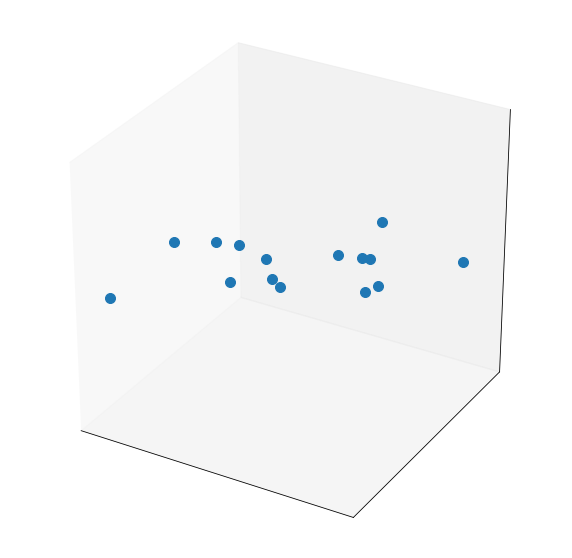
\includegraphics[scale=.4]{Imagenes/search1.png}}
\subfigure[Relaciones inducidas por los operadores de cambio]{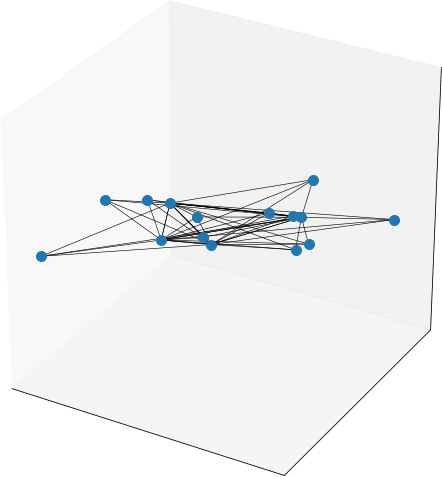
\includegraphics[scale=.4]{Imagenes/search2.png}}
\subfigure[Adición de la función de fitness]{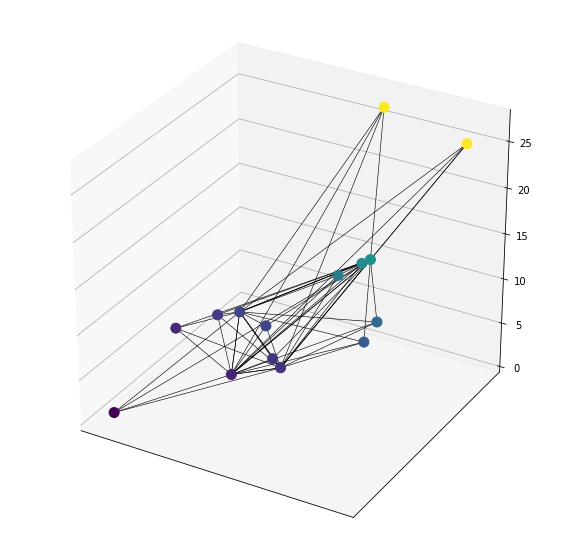
\includegraphics[scale=.4]{Imagenes/search3.png}}
\caption{Creación del paisaje de búsqueda}
\end{figure}

\begin{figure}[H]
\centering
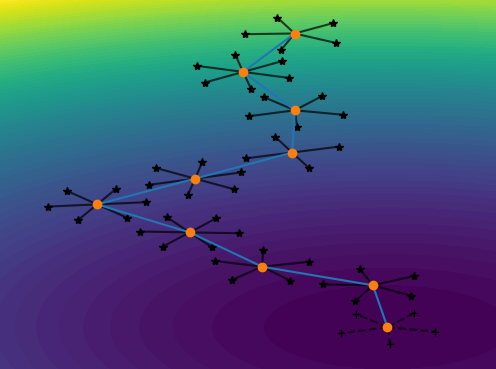
\includegraphics[scale=.5]{Imagenes/mettray.png}
\caption{Ilustración de una metaheurística de trayectoria.\\ En cada paso se selecciona un vecino mejor que la solución actual hasta que se cumple algún criterio de paro }
\end{figure}
% introducir ejemplos de mh de trayectoria
\subsection{Búsqueda Tabú}
Esta metaheurística de trayectoria es la que actualmente ha obtenido mejores resultados por lo que se describe a continuación:
% algoritmo

\section{Problema de planificación de producción tipo taller (JSP)}

Dentro de los problemas de planificación, el JSP modela un taller en el que hay $m$ máquinas, cada una de las cuales puede hacer varios tipos 
de procedimientos pero solo puede hacer uno de ellos a la vez. 
%
Se requiere completar $n$ trabajos, cada uno de los cuales está compuesto por $m$ operaciones, una por cada máquina en el taller, y que deben 
procesarse en un orden específico y por un tiempo específico en cada una de ellas. De este modo una operación solo puede comenzar a procesarse cuando su operación precedente en el trabajo y su operación precedente en la máquina ya han sido procesadas. Es decir que cada operación tiene dos tipos de dependencias, las propias de su trabajo y las de la máquina en donde ha de ser procesada.

Por ejemplo una panadería puede modelarse del siguiente modo; las herramientas como batidora, rodillo, horno, etc. pueden representarse como las
$m$ máquinas que se utilizan en un orden determinado para hacer $n$ distintos tipos de pan, los cuales pueden representarse como los trabajos 
a completar.

Las secuencias y tiempos de procesamiento para cada trabajo deben de especificarse para definir el problema. 
%
Habitualmente se presentan en una tabla de $n$ renglones por $m$ columnas esto se conoce como una instancia del JSP. 
%
Para cada renglón, las columnas contienen, de forma ordenada, la máquina en que debe procesarse el trabajo en cada paso y el tiempo 
que toma procesarlo. 
%
Por ejemplo en la tabla~\ref{tab:inst} se presenta una instancia del JSP con 3 máquinas y 2 trabajos. 
%
En esta instancia el trabajo 1 debe procesarse primero en la máquina 0 por 75 unidades de tiempo, luego en la máquina 2 por 54 unidades de tiempo y 
por último en la máquina 1 por 59 unidades de tiempo.

El problema a resolver consiste en hallar una planificación que sea óptima en algún sentido y respete los requisitos impuestos (orden y no concurrencia de diversas
operaciones).
%
Así, una planificación consiste en asignar tiempos de inicio y fin a cada operación respetando el orden requerido para cada trabajo. 

\subsection{Tipos de planificaciones}
Independientemente de cómo se representen o como se construyan, las planificaciones pueden clasificarse en varios conjuntos. Dentro del conjunto de planificaciones factibles se pueden distinguir tres subconjuntos de interés para el presente trabajo~\cite{sprecher1995semi}:
\begin{itemize}
    \item \textbf{Planificaciones semi-activas} Son aquellas en las que el tiempo de inicio de cada operación no puede disminuirse sin modificar el orden especificado en la planificación. De modo más intuitivo son aquellas en las que una máquina solo deja de trabajar porque la dependencia de la operación a procesar no ha sido procesada o porque ya terminó todo lo que tenía asignado.
    \item \textbf{Planificaciones activas} Son a su vez un subconjunto de las planificaciones activas y se definen como las planificaciones en las que no es posible disminuir el tiempo de inicio de ninguna operación sin aumentar el tiempo de inicio de otra. 
    \item \textbf{Planificaciones óptimas} Es el conjunto conformado por las planificaciones con el menor makespan posible. Este conjunto contiene planificaciones activas~\cite{Ponsich2013} aunque puede o no contener otras planificaciones que solo son factibles.
\end{itemize}

La relación entre estos conjuntos se ilustra en la figura \ref{fig:solspace}. 


\begin{figure}[H]
    \centering
    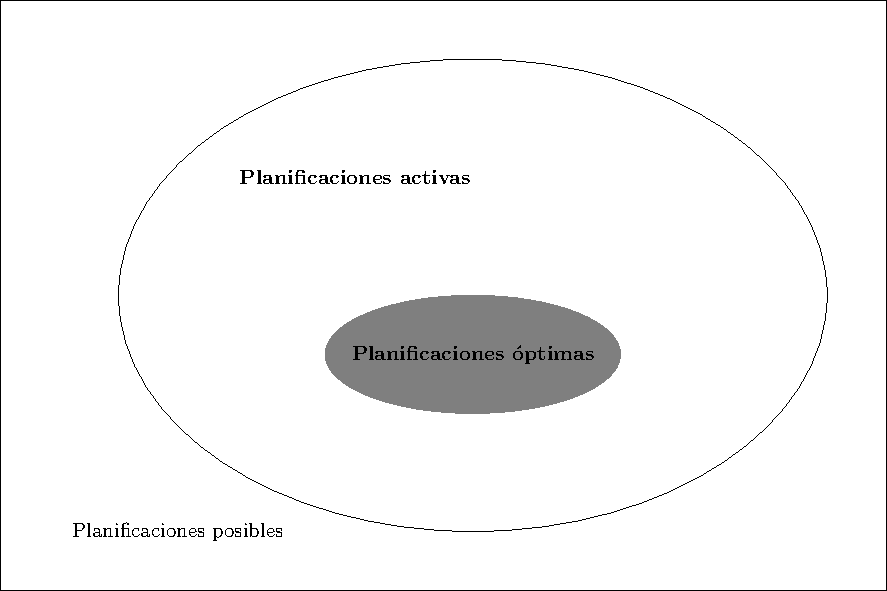
\includegraphics[scale=.8]{Imagenes/solspace.pdf}
    \caption{Subconjuntos de planificaciones. El área sombreada puede ser una intersección vacía}
    \label{fig:solspace}
\end{figure}

Es importante mencionar que el conjunto de las planificaciones factibles puede ser de tamaño arbitrario porque para cualquier planificación factible podemos insertar intervalos de tiempo inactivo de duración arbitraria entre operaciones en cualquier máquina sin alterar el cumplimento de las restricciones. Esto también implica que no hay una planificación única que cumpla que cumpla con algún orden determinado de las operaciones en cada máquina. En la literatura en general, así como en este trabajo, solo se considera el conjunto de planificaciones semi-activas lo cual elimina estos problemas. 
%
Otra ventaja de centrarnos en las planificaciones semi-activas es que nos permite definir el concepto \textbf{ruta crítica}. 

%
Para una planificación semi-activa una \textbf{ruta crítica} es una secuencia ordenada de $k$ operaciones $(O_1,O_2,\dots,O_k)$ que cumple con las siguientes propiedades: el tiempo de inicio de la primera operación es cero y el de finalización de la última es igual al makespan de la planificación, el tiempo de inicio de la operación $i$ es igual al tiempo de finalización de la operación $i-1$ para $i>1$ y la operación $i-1$ es una dependencia de la operación $i$ para $i>1$.  

%
La ruta crítica se compone a su vez de una serie de \textbf{bloques críticos} que consisten en las secuencias de operaciones de la ruta crítica que se ejecutan de forma 
adyacente en la misma máquina. 
%
Es importante mencionar que una planificación semi-activa siempre tiene al menos una ruta crítica pero puede tener más de una a la vez.
%
Existen varias formas de determinar si una planificación es óptima, como se explicará más adelante, pero la más usada es el tiempo que toma terminar la última operación.
%
A este tiempo se le conoce como \textbf{makespan}. 
%
Sin pérdida de generalidad nos restringimos al caso en el que el tiempo requerido para procesar cada operación es un entero positivo.

% x Indicar que surgen dos tipos de dependencias, una en las propias máquinas (no puedes empezar antes que tu predecesora), y otra entre trabajos (no puedes empezar
% x hasta que acabe de predecesor del trabajo).
% x Es difícil definir el concepto de ruta crítica, sin decir que se hace uso de soluciones semi-activas, entonces creo que es importante definir aquí ese concepto
% x Hay que ser más formal al definir la ruta crítica, algo así como secuencia de operaciones tales que cada una tiene dependencia con la anterior, en la que la primera 
% x empieza en el tiempo 0 de planificación y la última termina en el tiempo makespan, y que cumple además que, cada operación empieza justo al terminar la operación anterior de la secuencia

%
El siguiente ejemplo sirve para mostrar los conceptos antes presentados en un caso práctico y simple.

\subsection*{Ejemplo}
Se muestra un ejemplo de una instancia con 3 máquinas y 2 trabajos en la tabla \ref{tab:inst}.
\begin{table}[H]
\centering
\begin{tabular}{@{}llll@{}}
Trabajo & \multicolumn{3}{l}{\begin{tabular}[c]{@{}l@{}}Secuencia de procesamiento \\ (máquina, tiempo)\end{tabular}} \\ \midrule
0       & 0, 75                              & 2, 54                               & 1, 59                             \\ \midrule
1       & 0, 47                              & 2, 72                              & 1, 45   \\\hline                         
\end{tabular}
\caption{Instancia simple con 3 maquinas y 2 trabajos}
\label{tab:inst}
\end{table}

La siguiente es una posible planificación para la instancia de ejemplo, visualizada mediante un diagrama de gantt. En negro se marcan los trabajos que conforman la ruta crítica. 
\begin{figure}[H]
\centering
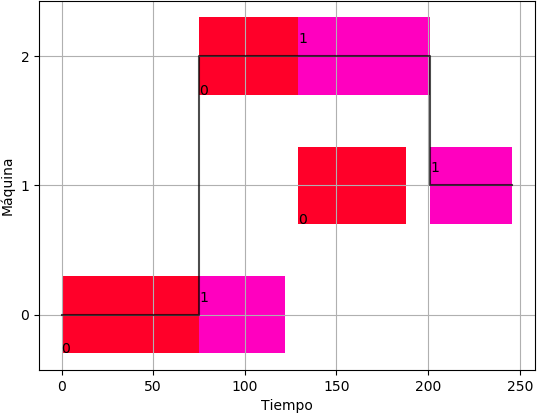
\includegraphics[scale=.7]{Imagenes/planejemplorc.png}
    \caption{Diagrama de gantt de una planificación posible para la instancia mostrada en la tabla \ref{tab:inst}. Se marcan los trabajos que pertenecen a la ruta crítica con una línea}
\label{fig:gantt}
\end{figure}

Si bien es conveniente visualizar una planificación mediante un diagrama de gantt como el mostrado anteriormente, resulta ventajoso representar computacionalmente 
estas planificaciones de otras formas. 
%
La representación de soluciones a un problema resulta ser una elección sumamente importante al momento de desarrollar, implementar y analizar los algoritmos que se 
propongan para resolver el problema~\cite{rothlauf2002representations}. 
%
En la siguiente sección se detallan dos formas de representación de especial importancia.

\subsection{Representación de planificaciones}
De manera general las representaciones para el JSP se pueden clasificar en\cite{Cheng1996}:
\begin{itemize}
    \item \textbf{Representación directa}: Se almacena el orden de los trabajos en cada máquina o sus tiempos de inicio y finalización.
    \item \textbf{Representación indirecta}: Se almacena información con la que se puede construir una planificación mediante un proceso de decodificación.
\end{itemize}

En este trabajo se utilizaron dos: una basada en permutaciones (representación directa) y las reglas de prioridad (representación indirecta).

\subsubsection*{Representación basada en permutaciones} 
En este modelo se identifica para cada máquina el conjunto de operaciones que deben procesarse en ella. Entonces una planificación se representa como un conjunto de $m$ permutaciones $(\sigma_0,\sigma_1,\dots,\sigma_m)$, donde $\sigma_i$ es la permutación de las operaciones que debe procesar la máquina $i$. Es decir que se asigna el orden de procesamiento de las operaciones cada máquina.
%
Esta representación no toma en cuenta el orden de procesamiento que deben cumplir las operaciones dentro de sus trabajos correspondientes por lo que no siempre representa planificaciones factibles.
%
Una forma de determinar si la permutación representa una planificación factible se construye un grafo dirigido $G=(V,A,E)$ en el que $V$ es un conjunto de nodos que representa las operaciones, las aristas $A$ representan la secuencia que deben seguir las operaciones dentro de un mismo trabajo y $E$ es otro conjunto de aristas que indica el orden de procesamiento en cada una de las máquinas. 

Pueden agregarse dos nodos de control que sirven como el nodo inicial o fuente del que dependen todas las operaciones ($S$) y final que depende de todos las operaciones ($*$), las restricciones de precedencia para las operaciones dentro de cada trabajo se representan como aristas dirigidas fijas llamadas aristas conjuntivas y las operaciones que deben procesarse en una misma máquina se unen mediante aristas llamadas disyuntivas cuya dirección se determina siguiendo la permutación dada. 
%
Para que una permutación represente una planificación factible su grafo asociado debe ser acíclico, puesto que la existencia de un ciclo en el grafo indica que hay una operación que está esperando a que se procese alguna otra operación que a su vez depende de que se procese la primera.
%
Una vez que se sabe que el grafo es acíclico se puede proceder a asignar tiempos de inicio y fin a cada operación asignando al nodo fuente ($S$) tiempo de inicio y finalización igual a cero y marcándolo como visitado. Posteriormente aplicando un algoritmo para recorrer el grafo cerciorándonos de solo visitar un nodo cuando ambas de sus dependencias han sido visitadas y asignarle un tiempo de inicio mayor que el mayor tiempo de finalización de sus dependencias y un tiempo de finalización igual al tiempo inicial más la duración de la misma.

Si se busca generar una planificación semi-activa, entonces el tiempo de inicio de la operación será el máximo de los tiempos de finalización de sus dependencias.

\subsubsection*{Ejemplo}
La planificación mostrada en la figura \ref{fig:gantt} tendría la siguiente representación como permutaciones:
\begin{align*}
\sigma_0 &= (O_{0,0}\,,\,O_{1,0})\\
\sigma_1 &= (O_{0,2}\,,\,O_{0,1})\\
\sigma_2 &= (O_{0,1}\,,\,O_{1,1})
\end{align*}
A partir de estas permutaciones se construye el grafo antes descrito y se escogen las direcciones de las aristas disyuntivas como se muestra en la figura \ref{fig:dgraph}. En este caso se verifica que el grafo es acíclico como 
\begin{figure}[H]
    \centering
    \begin{subfigure}{.8\textwidth}
        \centering
        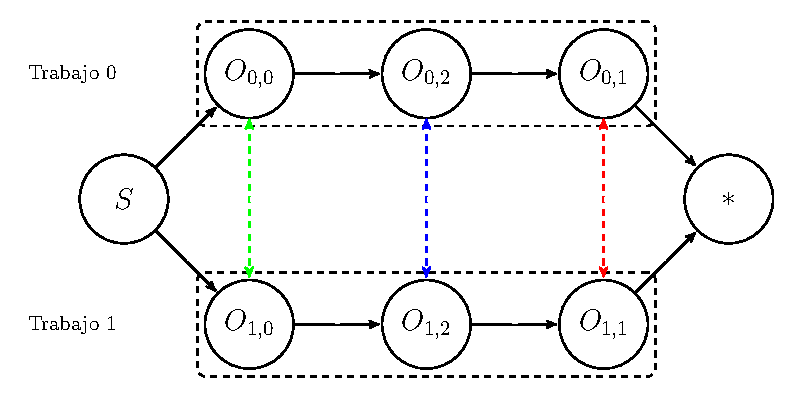
\includegraphics[width=.8\linewidth]{Imagenes/disyuntive.pdf}
        \caption{Representación de una instancia, los colores distinguen entre las tres máquinas.}
    \end{subfigure}
    \begin{subfigure}{.8\textwidth}
        \centering
        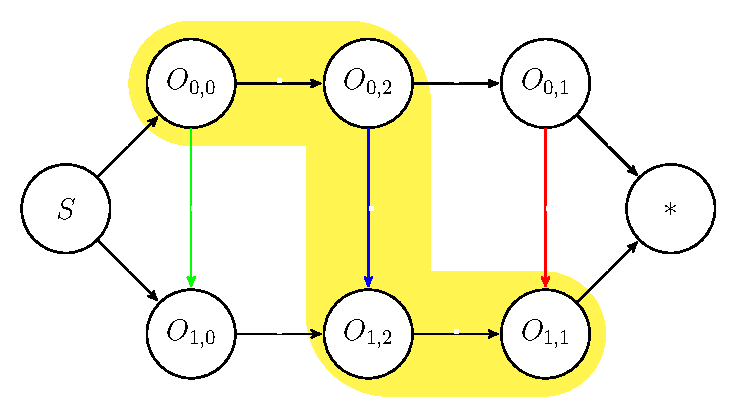
\includegraphics[width=.8\linewidth]{Imagenes/plandisyuntive.pdf}
        \caption{Planificación obtenida al fijar las aristas disyuntivas como en \ref{fig:gantt}. La ruta critica se resalta en amarillo}
    \end{subfigure}
\caption{Modelo de grafo disyuntivo para la instancia de ejemplo \ref{tab:inst}}
        \label{fig:dgraph}
\end{figure}

\subsubsection*{Representación basada en reglas de prioridad}
En esta representación una planificación se construye al aplicar un proceso de simulación en el que para cada maquina se construye una cola con las operaciones cuyas dependencias ya han sido procesadas. Inicialmente se tienen en las colas solo las operaciones iniciales de cada trabajo. Una vez que se tiene esto se utiliza una regla de prioridad para elegir qué operación debe planificarse en qué máquina. Se actualizan las colas para las máquinas que lo requieran y se continua con este proceso hasta completar la planificación (vaciar las colas).

Existen muchas reglas de prioridad que toman en cuenta cosas como la duración de la operación, la cantidad de operaciones restantes, la duración del trabajo al que pertenece una operación, entre muchas otras. La calidad de la planificación construida depende de la regla de prioridad que se utilice y de la estructura de la instancia en sí.


%Como se juntan las definiciones con lo demas
\section{Metaheurísticas aplicadas al JSP}
La complejidad del JSP hace que las metaheurísticas sean actualmente los métodos más utilizados para resolver instancias grandes. Estas han conseguido hallar buenas soluciones para los conjuntos de prueba más populares. Aunque se han propuesto muchas metaheurísticas, práticamente todas utilizan el concepto de vecindad. Como ya se explicó, la definición de una estructura de vecindad es parte del paisaje de búsqueda y tiene un gran impacto en los resultados obtenidos. Desde que se propuso la primera vecindad en 1996, se han propuesto veecindades cada vez con mejores resultados.

\subsection*{Vecindades previamente propuestas}
Se han propuesto varias estructuras de vecindad al JSP, a continuación se describen las más importantes a la fecha:

\begin{itemize}
\item N1 \cite{blazewicz1996job} Consiste en considerar todas las soluciones que se crean al intercambiar cualquier par de operaciones adyacentes que pertenecen a un bloque crítico. Esta vecindad es muy grande y considera muchos cambios que no mejoran el makespan.
\begin{figure}[H]
\centering
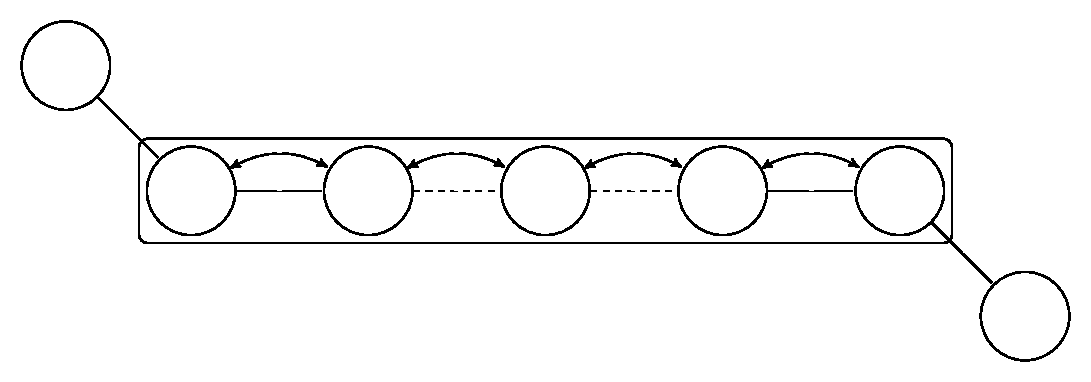
\includegraphics[scale=.7]{Imagenes/N1.pdf}
\caption{Movimientos de la vecindad N1}
\end{figure}

\item N4 \cite{dell1993applying} Esta vecindad se propuso como un refinamiento y extensión de la vecindad N1 y toma como base el concepto de bloque crítico. Consiste en llevar operaciones internas del bloque crítico al inicio o final. 
\begin{figure}[H]
\centering
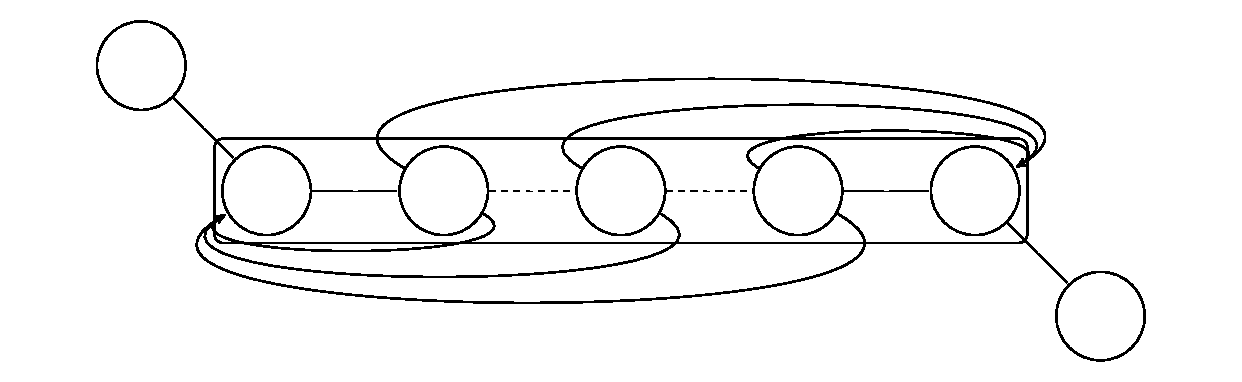
\includegraphics[scale=.7]{Imagenes/N4.pdf}
\caption{Movimientos de la vecindad N4}
\end{figure}


\item N5 \cite{EugeniuszNowicki2003} Consiste en intercambiar solo las operaciones adyacentes a la final o inicial de un bloque crítico.  
\begin{figure}[H]
\centering
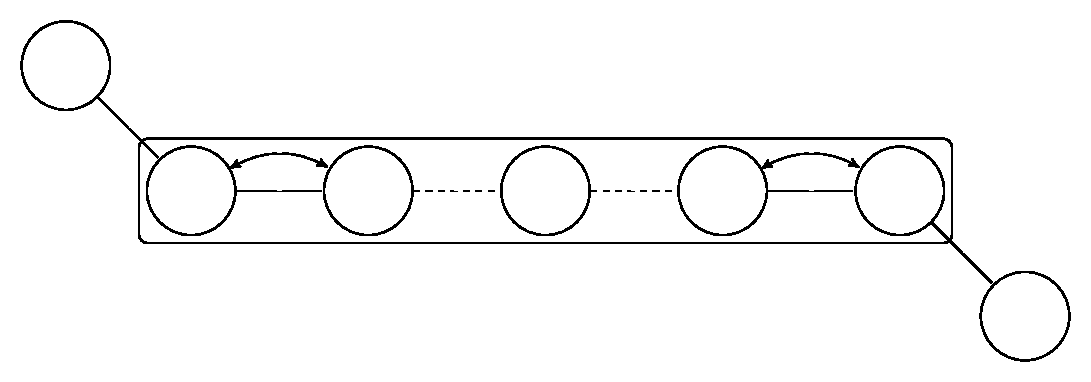
\includegraphics[scale=.7]{Imagenes/N5.pdf}
\caption{Movimientos de la vecindad N5}
\end{figure}

\item N6 \cite{Balas1998} Los autores utilizan varios teoremas para identificar pares $(u,v)$ de operaciones dentro de un bloque crítico que puedan llevar a mejorar la solución y a su vez identificar si se tiene que mover a $u$ justo después de $v$(forward) o bien a $v$ justo antes de $u$ (backward).
\begin{figure}[H]
\centering
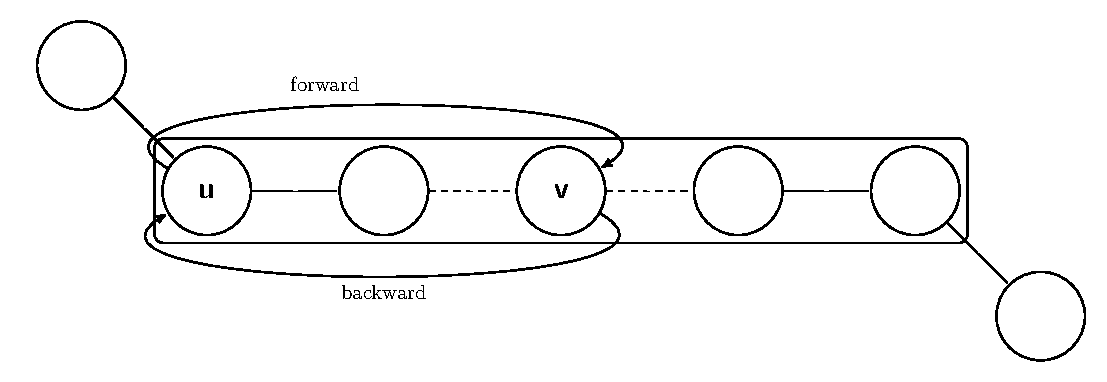
\includegraphics[scale=.7]{Imagenes/N6.pdf}
\caption{Los dos tipos de movimientos para un par $(u,v)$}
\end{figure}

\item N7 \cite{Zhang2007} Esta vecindad se plantea como una extensión de la N6 en la cual se toma la idea de los movimientos entre pares de operaciones de un bloque crítico. Los autores toman en cuenta todos los cambios posibles entre el inicio o fin del bloque crítico con todas las operaciones internas.

\begin{figure}[H]
\centering
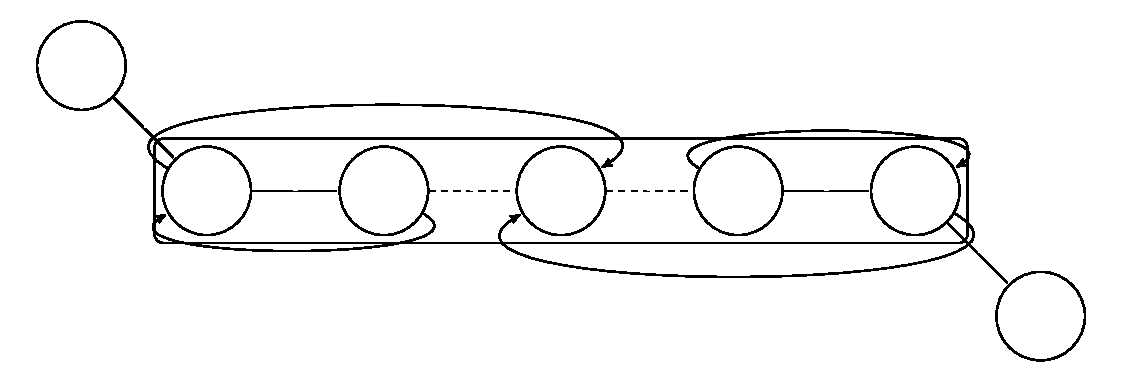
\includegraphics[scale=.7]{Imagenes/N7.pdf}
\caption{Movimientos de la vecindad N7}
\end{figure}
\end{itemize}

Las vecindades antes presentadas se han centrado en operaciones que pertenecen a la ruta crítica por varias razones, la vecindad resultante es suficientemente pequeña como para ser explorada en su totalidad, el makespan de una planificación solo puede reducirse haciendo cambios en la ruta crítica y pueden garantizarse que cualquier vecino representa una solución factible.\\

La literatura reciente se ha centrado en hacer los algoritmos existentes más eficientes dejando de lado la parte de la representación o de la función de fitness. Existen otras ideas que no se han explorado a fondo pero parecen prometedoras como proponer extensiones a alguna de las vecindades, cambiar la representación y proponer una función de fitness que no solo tome en cuenta el makespan de modo que tengamos más formas de diferenciar entre soluciones. En la siguiente sección se presentan algunas otras medidas de calidad para planificaciones del JSP.
% ve como se pueden mejorar 
\subsection*{Criterios de optimalidad}
Como ya se ha mencionado el criterio de optimalidad más usado es el makespan, no obstante existen muchos otros criterios de optimalidad que pueden usarse para asignar un valor de fitness a una planificación. 

Si denotamos por $C_i$ al tiempo de finalización del trabajo $J_i$ y $f_i(C_i)$ a su costo asociado, podemos distinguir dos tipos de funciones de costo en la literatura\cite{Brucker2001}:
\[f_{\max}:=\max\{f_i(C_i)\}\]
y 
\[\sum f_i(C):=\sum_{1\leq i\leq n}f_i(C_i)\]

Los costos asociados a cada uno de los tiempos de finalización de los trabajos pueden tomar muchas formas, por ejemplo pueden introducirse pesos para cada trabajo o fijar tiempos de finalización esperado para cada trabajo y medir la desviación de ellos.

Dependiendo del problema en sí, puede ser que se le de más o menos valor a distintos aspectos de la planificación como el tiempo que están detenidas las máquinas, o el tiempo que tarda un trabajo en particular. El makespan se ha extendido como criterio de optimalidad porque está muy relacionado con los costos económicos de la planifacición\cite{Rand1977}.


Con las definiciones anteriores sobre vecindades, función objetivo y representaciones de las soluciones podemos construir el paisaje de búsqueda para el JSP. 
\section{Paisaje de búsqueda del JSP}

La estructura del paisaje de búsqueda influye de manera determiante en el éxito o fracaso de las metaheurísticas. Dependiendo de la <<forma>> que tenga el paisaje se favorecera el uso de ciertas metaheurísticas. La <<forma>> del paisaje hace referencia a cómo cambia el valor de fitness para soluciones conectadas entre sí. Dos medidas que son generalmente utlizadas para esto miden cómo cambia el valor de la función de fitness conforme nos acercamos a un óptimo local y la otra mide qué tanto cambia el fitness entre soluciones vecinas\cite{skauffman}. La primera de estas medidas nos da una idea de qué tan grandes son los valles que rodean a un mínimo local si es que existen y la segunda nos da una ida de la rugosidad del paisaje.

% imagen
\begin{figure}[H]
    \centering
    \subfigure[Paisaje rugoso con muchos óptimos locales]{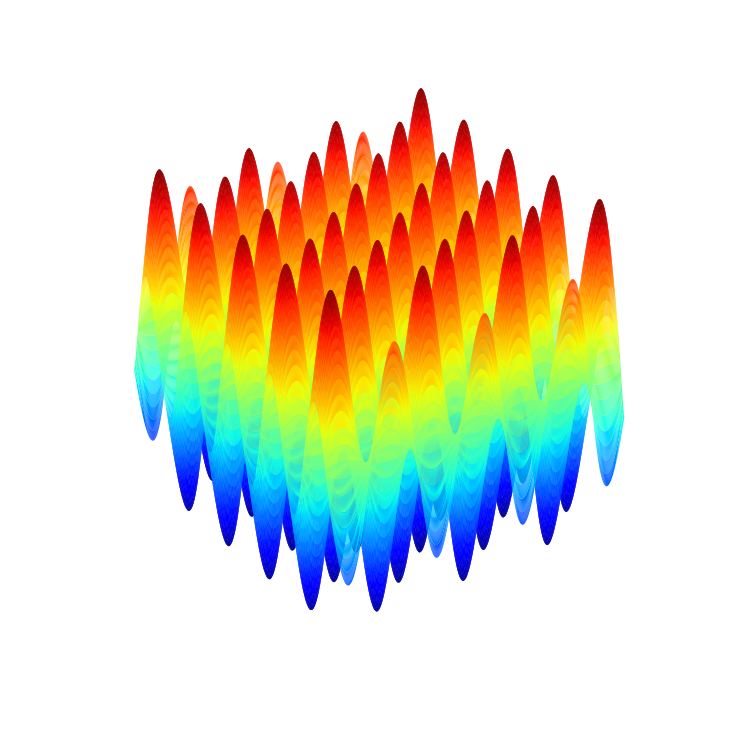
\includegraphics[scale=.3]{Imagenes/rugged.png}}
    \subfigure[Paisaje rugoso con con un gran valle]{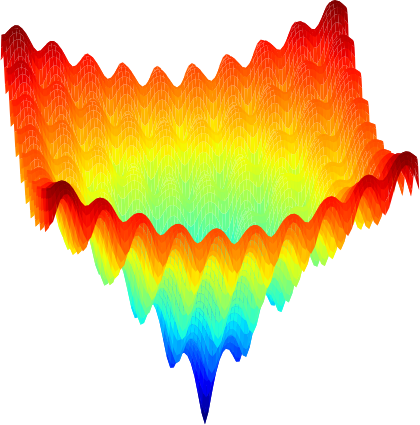
\includegraphics[scale=.3]{Imagenes/ruggedvalley.png}}
    \subfigure[Paisaje suave con un gran valle]{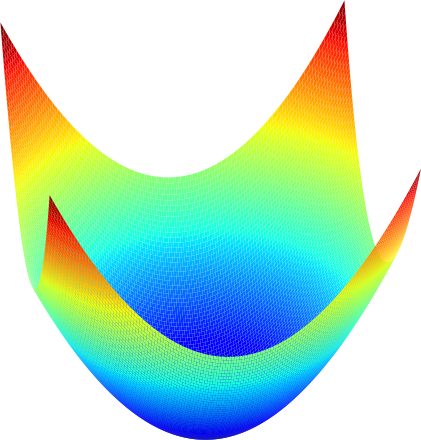
\includegraphics[scale=.3]{Imagenes/smoothvalley.png}}
    \caption{Diferentes tipos de paisajes de búsqueda. Se muestran paisajes continuos con fines ilustratios}
\end{figure}

En el caso del JSP se ha encontrado que el paisaje de búsqueda para una instancia al azar tiende a ser muy dependiente de la razón entre el número de máquinas y número de trabajos de la misma \cite{Streeter2006}. También se ha observado que el paisaje tiende a tener muchos óptimos locales de baja calidad para instancias dificiles \cite{mattfeld1999search} y que en general algunas soluciones están mucho mas conectadas que otras \cite{bierwirth2004landscape}. 

Estas características explican en parte por qué los métodos basados en búsqueda local como la búsqueda tabú combinados con métodos sofisticados de exploración han tenido tan buenos resultados. Puede ser que las soluciones que esten más conectadas a otras sean de baja calidad y sea necesario evitar ser <<atraidos>> hacia ellas para llegar a soluciones de mejor calidad.

En este sentido, podemos pensar que para que una metaheurística basada en búsqueda local tenga mayor probabilidad de encontrar buenas soluciones debemos plantear el paisaje de búsqueda de modo que no nos atasquemos en óptimos locales de mala calidad, ya sea porque están muy conectados y funcionan como atractores o bien porque el paisaje de búsqueda es tan rugoso que hay óptimos locales por doquier.

\newpage

\chapter{Propuestas}\label{cap:prop}
\section{Vecindad basada en soluciones activas}
Esta vecindad surge del cambio de representación propuesto. En cada paso del algoritmo para construir una solución activa se consideran varias operaciones que <<compiten>> para ser planificadas (i.e. son planificables en ese momento) de las cuales se elige la que tiene la llave de mayor valor numérico. 

La idea es construir la vecindad a partir de estas operaciones que compiten. En un principio puede pensarse en considerar todos los posibles ordenamientos posibles para dichas operaciones pero esto da lugar a una vecindad demasiado grande por lo que se considera únicamente hacer cambios por pares de llaves entre la operación elegida y todas sus competidoras.
\begin{figure}[H]
\centering
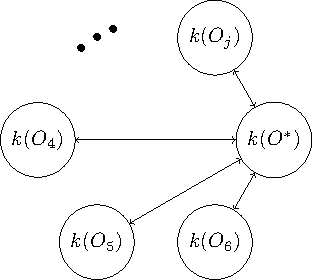
\includegraphics[scale=1.3]{Imagenes/vec2.pdf}
\caption{Movimientos de la vecindad propuesta. $k(O^*)$ es la llave de la operación elegida, las flechas representan los posibles intercambios entre las $j$ operaciones competidoras.}
\end{figure}
%diagrama

El tamaño de esta vecindad puede ser bastante grande ya que para cada paso del algoritmo \ref{alg:GT} se tienen tantos movimientos como operaciones competidoras, las cuales pueden ir desde 1 hasta el número de trabajos $n$ siendo en el peor caso de tamaño $O(nm*n)$. Como se mostará mas adelante en la validación experimental, en realidad el número de operaciones que compiten por lo general es solo una fracción pequeña de $n$ con lo que la vecindad puede manejarse sin problemas.


Los movimientos de esta vecindad pueden generar soluciones muy diferentes dependiendo de dónde se encuentren en la planificación las operaciones consideradas. Si se cambia la llave de una operación que fue planificada al principio puede ser que la solución cambie en muchos otros lugares porque el conjunto de operaciones disponibles puede llegar a ser completamente distinto al llegar a un paso más avanzado en la construcción de la solución. 

\section{Extensión a vecindad N7}
Como punto de partida se planteó agregar movimientos a la vecindad N7 con la cual se han obtenido los resultados del estado del arte.
Los movimientos que plantea esta vecindad solo tienen que ver con pares de operaciones en la ruta crítica por lo que una extensión sencilla consiste en considerar movimientos de operaciones que pueden no pertenecer a la ruta crítica.

Es importante resaltar que si no se planteara también una función de fitness que no tome solo en cuenta el makespan estos movimientos podrían nunca llevarían a una mejora \cite{blazewicz1996job}. 
Los movimientos planteados se basan en observar que en alguna solución encontrada por una búsqueda local para cada maquina pueden existir periodos de tiempo en la que está inactiva pero existe alguna operación en la ruta critica que podría comenzar a procesarse en este periodo y que se procesa después. Ninguna de las vecindades previamente propuestas considera movimientos de las operaciones de la ruta crítica más allá del bloque crítico por lo que estos movimientos representan un conjunto previamente no explorado de soluciones.

Intuitivamente lo que se pretende es llenar un <<hueco>> en la planificación con una operación de un bloque crítico.

\begin{figure}[H]
\centering
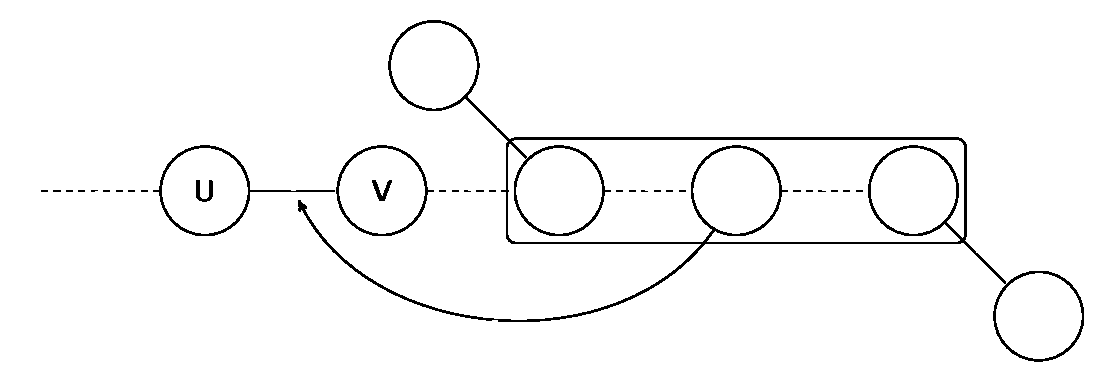
\includegraphics[scale=.7]{Imagenes/N8.pdf}
    \caption{Movimientos propuestos. El tiempo de inicio de \textbf{v} es mayor al de finalización de \textbf{u}}
\end{figure}

En general esta vecindad resulta de un tamaño muy reducido porque existen muchos movimientos que hacen que la solución resultante sea infactible. 

\section{Función de fitness}\label{prop:fitness}
La función de fitness es el elemento del paisaje de búsqueda al que se han reportado menos modificaciones en la literatura. 
%
En general cuando se utilizan otros criterios de optimalidad el problema se convierte en uno de optimización 
multi-objetivo~\cite{gong2019effective,sakawa2000fuzzy,ponnambalam2001multiobjective}.
%
En~\cite{uckun1993managing} se propuso optimizar el makespan pero tomando en cuenta exclusivamente el tiempo inactivo en la planificación 
aunque los resultados no fueron muy alentadores.   

La propuesta presentada en este trabajo consiste en construir un arreglo de características para cada planificación de modo que puedan 
compararse lexicográficamente. 
%
La idea principal es tener una forma de distinguir entre soluciones con el mismo makespan, lo que puede ayudar a atravesar regiones que de 
otro modo serían <<planas>> y que para una búsqueda local representarían un punto de paro. 
%
En el mejor de los casos la adición de estas cantidades no solo nos permitiría atravesar planicies sino que también serviría como guía para
mantener una planificación que no sea propensa a estancarse prematuramente en un óptimo local de mala calidad.

Para plantear las características para este arreglo se tomaron en cuenta otros criterios de optimalidad hallados en la literatura así como propuestas 
propias que se hallaron empíricamente. 
%
También se planteó considerar todos los tiempos de finalización de las máquinas ordenados de mayor a menor.
%
Las características tomadas en cuenta fueron las siguientes ($J_i$ es el tiempo de finalización del trabajo $i$ y $C_i$ el tiempo de finalización de la máquina $i$):
\begin{itemize}
    \item $\mathbf{C_{max} = \max{C_i}}$ : Este es el criterio de optimalidad más usado y el más ampliamente reportado en la literatura. 
    \item $\mathbf{\sum C_i^2}$: La ventaja de esta medida es que toma en cuenta todos los tiempos de finalización de las máquinas y al elevar al cuadrado, 
		las que toman más tiempo en acabar contribuyen mucho más que las que toman poco tiempo. Con esta medida podemos distinguir entre dos soluciones con el mismo makespan 
		pero en la que se ha mejorado el tiempo de alguna máquina, especialmente si es una de las máquinas que tardaba más en terminar.
    \item $\mathbf{\sum J_i}$: También conocido como \textit{Flowtime}, mide los tiempos de finalización de los trabajos y puede llevar a encontrar mejoras en distintas 
		máquinas a la vez.
    \item $\mathbf{\sum I(C_i=C_{max})}$: Número de máquinas cuyo tiempo de finalización es igual al makespan. Conforme aumenta el número de máquinas que cumplen esta 
		condición, parece menos probable que un solo cambio contribuya a mejorar el makespan ya que se tendría que reducir a la vez el tiempo de todas ellas. 
    \item \textbf{Número de rutas críticas}. Esta medida está directamente relacionada con la anterior pero puede tener la ventaja de poder hacer cambios progresivos 
		para eliminar las rutas críticas, aunque eso no implique reducir el tiempo final de alguna máquina, y así lograr una mejora en el makespan. 
    \item $\mathbf{Var(C_i)}$ Varianza de los tiempos de finalización. Esta medida es parecida a la suma de tiempos de finalización al cuadrado pero en este caso se 
		mide la distancia a la duración promedio por lo que no solo se centra en las máquinas que tardan más sino también en las que se tardan menos. Esto puede ayudar a 
		que no se planifiquen operaciones en un solo subconjunto de máquinas mientras que las otras permanecen en espera.
    \item $\mathbf{(\{C_i\})}$ Tupla de tiempos de finalización ordenados. Esta tupla engloba de cierto modo varias de las características previamente mencionadas pero
		tiene la ventaja de requerir menos trabajo computacional para construir al solo ser necesario ordenar cantidades ya conocidas.
\end{itemize}

Estas características se combinaron de varias formas como se mostrará en la validación experimental. 

\section{Representación de soluciones activas basada en llaves aleatorias}
La representación propuesta se basa en asignar a cada operación un número real entre 0 y 1 el cual sirve para definir un orden entre 
operaciones en una misma máquina mediante un proceso de decodificación similar al planteado en~\cite{bean1994genetic,norman1996random,Ponsich2013}.
%
Para decodificar la solución a partir de las llaves se utiliza el algoritmo de Giffler \& Thompson \cite{Giffler1960} con el cual se generan 
soluciones activas.

Una consecuencia importante de este cambio en la representación es que el espacio de búsqueda se reduce a solo las soluciones activas y como se sabe 
existen soluciones activas entre las óptimas, esta representación puede encontrar una solución óptima buscando sólo en un subconjunto de todas las
soluciones.

Un punto negativo es que esta representación es n a 1 porque solo importa el valor relativo de las llaves que compiten entre sí, es decir qué diferentes 
valores de llaves pueden llevarnos a la misma solución. 
%
En principio no parece un problema muy grave, pero hay que tenerlo en cuenta a la hora de diseñar los operadores de movimientos, para no quedarse
estancado en movimientos que vuelven a generar exactamente la misma solución.

A continuación se presenta el algoritmo para construir planificaciones activas de llaves numéricas.

\subsection{Algoritmo de Giffler \& Thompson}
Para explicar el algoritmo de Giffler \& Thompson se adoptan las siguientes notaciones:
\begin{itemize}
    \item $O_i$ la operación $i$.
    \item $M(O_i)$ la máquina en la que debe procesarse la operación $O_i$.
    \item $t_f(O_i)$ el tiempo en que se terminaría de procesar la operación $O_i$ si se planifica en este paso.
    \item $t_i(O_i)$ el tiempo en que se comenzaría a procesar la operación $O_i$ si se planifica en este paso.
    \item $k(O_i)\in [0,1]$ el valor de la llave asignada a $O_i$.
\end{itemize}

El primer paso es marcar como planificable la primera operación de cada trabajo. 
%
Posteriormente se identifica, de entre las operaciones planificables, la operación $O_{min}$ con el menor tiempo de finalización si se planificase en 
este paso y la máquina $M^*=M(O_{min})$ en la cuál debe procesarse. 
%
Nótese que si en esa máquina, se planificara a continuación una operación que empezase después de ese tiempo, no se tendría una solución activa.
%
Por ello, se toma dicho tiempo de finalización $t^*_f = t_f(O_{min})$, y se escoge alguna de las operaciones planificables en $M^*$ cuyo tiempo de inicio sea menor
a $t^*_f$ y se planifica.
%
A continuación se actualizan las operaciones planificables y este proceso se repite hasta completar la planificación. 
%
El algoritmo es el siguiente:

\begin{algorithm}[H]
 \KwData{Instancia del JSP}
 \KwResult{Planificación activa}
 Inicializar el conjunto de operaciones planificables $\Omega$\;
 \While{$\Omega$ no vacío}{
    Determinar la operación con el menor tiempo potencial de finalización $O_{min}=\arg\min_{O\in\Omega} \,\,t_f(O)$ \;
    Determinar el tiempo de finalización $t^*_f$ y la máquina $M^*$ en que se procesa $O_{min}$\;
    Identificar el conjunto $C\subset\Omega$ de operaciones que cumplen $t_i(O) < t^*_f$ y $M(O)=M^*$\;
    Escoger la operación $O^*\in C$ que tenga asignada la llave de mayor valor\;
    Asignar tiempo de inicio y fin a $O^*$\;
    Actualizar $\Omega$ eliminando a $O^*$ y agregando a su sucesora si existe\;
 }
    \label{alg:GT}
    \caption{Algoritmo de Giffler \& Thompson}
\end{algorithm}
\subsubsection*{Ejemplo}
Como ejemplo ilustrativo se muestran los primeros pasos para construir la planificación mostrada en la figura \ref{fig:gantt} asociada 
a la instancia de ejemplo mostrada en la tabla \ref{tab:inst}.

Para recuperar la planificación previamente mostrada se asignan las llaves de la siguiente manera: \[k(O_{00})=k(O_{01})=k(O_{02})=1\]  \[k(O_{10})=k(O_{11})=k(O_{12})=0\]
\begin{itemize}
    \item Se inicializa $\Omega$ agregando las operaciones iniciales de cada trabajo, es decir:

\[\Omega = \{O_{10},O_{00}\}\]

     \item Se identifica a la operación que acabaría primero si se planifica ya, en este caso es $O_{10}$ que se debe procesar en la máquina $M_0$. 

     \item Se identifican las operaciones que podrían comenzar a procesarse antes del tiempo potencial de finalización de $O_{10}$. 
		 En este caso solo $O_{00}$ y  $O_{10}$ cumplen las condiciones.

Como $k(O_{00})>k(O_{10})$ se planifica $O_{00}$ se le asignan $0$ y $54$ como tiempos inicial y final.

     \item Se actualiza $\Omega$ eliminando a la operación planificada y agregando a su sucesora $O_{02}$.

\[\Omega\leftarrow \{O_{10},O_{02}\}\]
\end{itemize}
Este proceso continua de acuerdo al algoritmo \ref{alg:GT} hasta que todas las operaciones se encuentren planificadas.

\subsection{Construcción de soluciones activas a partir de no activas}

Realizar una búsqueda a partir de soluciones activas tiene la ventajas de moverse entre soluciones con una calidad media
superior.
%
Sin embargo, el proceso de generar las soluciones es costoso, por lo que tiene el inconveniente de analizar una menor
cantidad de soluciones candidatas, con respecto al caso en que no se aseguran que las soluciones son activas.
%
Por ello, es posible que utilizar un esquema en que se usen ambos tipos de representaciones de forma simultánea sea
ventajoso.
%
Con este fin, de diseñó una forma para movernos movernos entre soluciones de ambas representaciones, en concreto, para
generar una solución activa y su representación basada en llaves, a partir de una solución previa que no tiene que ser activa. 

%TODO: cambiar y directamente hablar de las permutaciones tal y como se hizo en el capítulo 2.
Como se vio en el modelo de grafo disyuntivo, construir una planificación consiste en elegir direcciones de aristas disyuntivas. 
%
Esto al final genera un orden para las operaciones en cada máquina i.e., una permutación. 
%
Para hallar la representación de alguna de estas soluciones en el esquema propuesto se toma esta permutación de las operaciones para cada máquina 
y se le asigna a cada una una prioridad decreciente acuerdo a su posición en la permutación.
\[k(O_i)>k(O_{i+1})\]
\[\text{donde }O_i\text{ es la operación número $i$ en procesarse}\]

Esta asignación nos asegura que se mantenga el orden de muchas operaciones pero convierte a la solución en activa. 
%
A continuación se muestra un ejemplo ilustrativo.

\subsubsection*{Ejemplo}
Consideremos la instancia del JSP mostrada en la siguiente tabla:
\begin{table}[H]
\centering
\begin{tabular}{@{}llll@{}}
Trabajo & \multicolumn{3}{l}{\begin{tabular}[c]{@{}l@{}}Secuencia de procesamiento \\ (máquina, tiempo)\end{tabular}} \\ \midrule
0 & 1, 37 & 0, 13 & 2, 35\\ \midrule
1 & 0, 8 & 1, 4 & 2, 9 \\\hline                         
2 & 1, 34 & 2, 72 & 0, 96 \\\hline                         
3 & 1, 63 & 0, 77 & 2, 24 \\\hline                         
\end{tabular}
\caption{Instancia 3 maquinas y 4 trabajos}
\label{tab:instactive}
\end{table}

La siguiente figura muestra un diagrama de gantt para una posible planificación.

\begin{figure}[H]
     \centering
     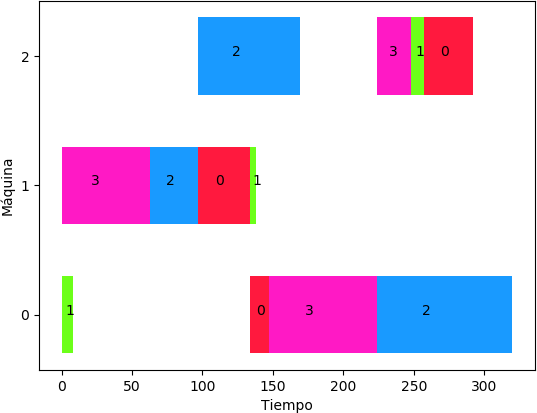
\includegraphics[scale=.7]{Imagenes/ganttnonactivepr.png}
     \caption{Planificación posible para la instancia en \ref{tab:instactive}. }
     \label{fig:nonactivepr}
\end{figure}
A partir de la planificación mostrada podemos asignar las prioridades del modo previamente dicho con lo que después de construir la planificación a partir de estas prioridades obtenemos la planificación que se muestra en la siguiente figura.
\begin{figure}[H]
     \centering
     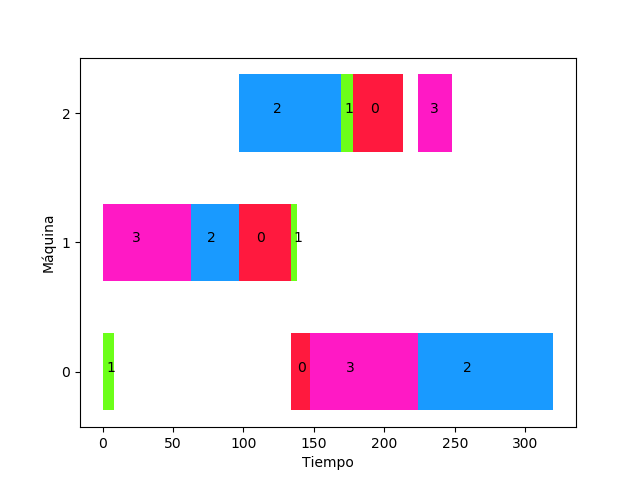
\includegraphics[scale=.7]{Imagenes/ganttactivepr.png}
     \label{fig:activepr}
     \caption{Planificación activa reconstruida a partir de la mostrada en \ref{fig:nonactivepr}}
\end{figure}

Podemos notar como dos operaciones cambian de lugar de modo que se planifican antes sin aumentar el tiempo de inicio de otras.

Una característica importante de esta representación es que el algoritmo usado para decodificar una solución activa a partir de las llaves numéricas considera en cada paso varias operaciones candidatas a planificar que cumplen con los criterios antes mencionados. Estas operaciones son la pieza en la que se basa la siguiente propuesta para una estructura de vecindad.


\chapter{Validación experimental}
% capitulo validacion experimental
En este trabajo se ponen a prueba las modificaciones planteadas al comparar los resultados obtenidos con los mejores reportados en la literatura hasta la fecha.

Las modificaciones se presentan en el siguiente orden: en primer lugar se presentan los resultados de búsqueda local con la vecindad N7 y con función de fitness igual al makespan, es decir que el único cambio es en la metaheurística utilizada para tener una linea base. En segundo lugar se presentan las modificaciones hechas a la función de fitness. Posteriormente se presentan los resultados de la extensión a la vecindad N7. Por último se presentan los resultados del cambio de representación junto con la nueva estructura de vecindad basada en soluciones activas.

Cada una de las variaciones propuestas se ejecutó 50 veces para cada instancia para obtener un conjunto de resultados que podemos comparar.

Los resultados se muestran de modo que las modifcaciones se van agregando para mejorar el desempeño del algoritmo. Primero se presenta el cambio en metaheurística seguido del cambio en la función de fitness posteriormente se considera la extensión de vecindad planteada y por último el cambio de representación. El orden es el siguiente:
\begin{enumerate}
    \item ILS con vecindad N7 y makespan como función de fitness.
    \item ILS con diferentes funciones de fitness.
    \item ILS con extensión de vecindad N7.
    \item ILS con la representación y vecindades propuestas.
\end{enumerate}
\section{ILS con vecindad N7}
Estos resultados sirven como una base para determinar si las modificaciones posteriores resultan en mejoras apreciables.

Se muestran los resultados de manera gráfica para facilitar su visualización. Los resultados detallados se encuentran en el apéndice \ref{app:resn7ils}. Para cada instancia se muestra la mediana del error relativo de los resultados con respecto a los mejores resultados reportados en la literatura mostrados en el apéndice \ref{tab:sota}. 

\begin{figure}[H]
    \begin{subfigure}{\textwidth}
        \centering
        %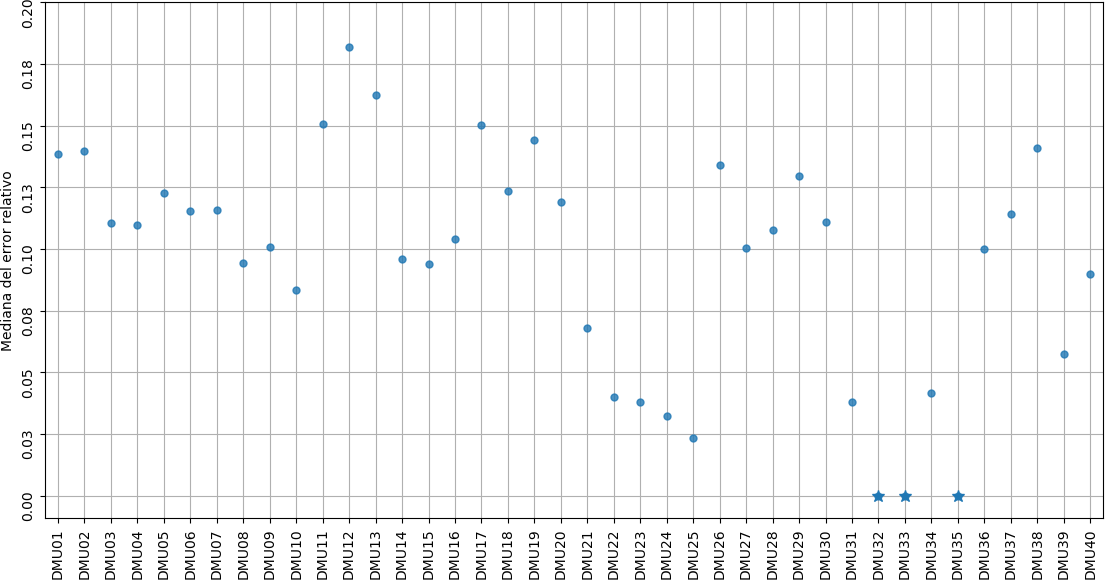
\includegraphics[height=.78\textwidth,width=.95\textheight,angle=270]{Imagenes/resn7ils1.png}
        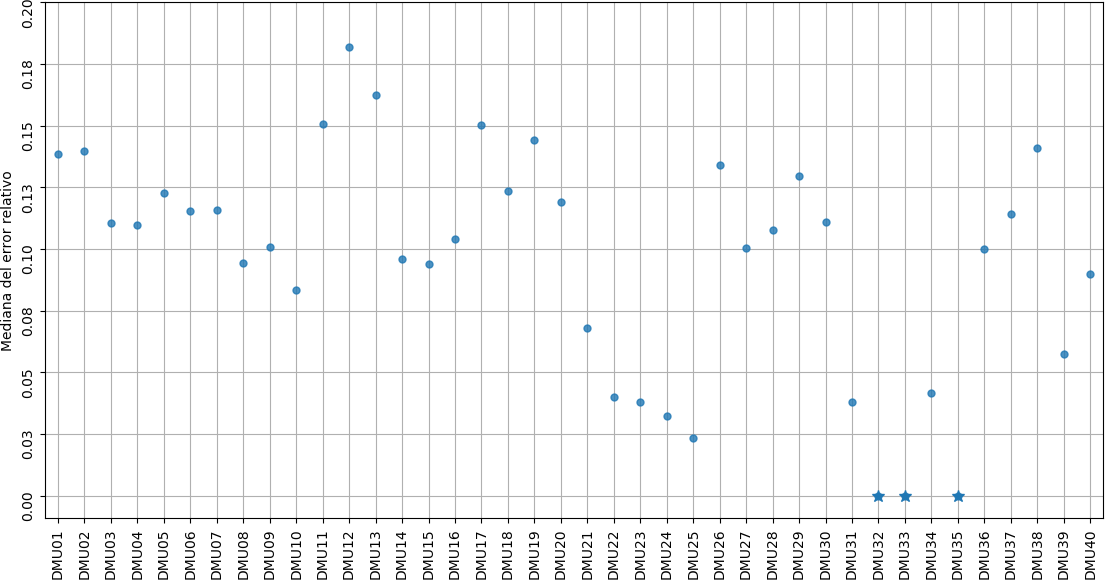
\includegraphics[scale=.65]{Imagenes/resn7ils1.png}
        \caption{Resultados para las instancias \textbf{DMU01-40}}
    \end{subfigure}
\end{figure}
\begin{figure}[H]\ContinuedFloat
    \begin{subfigure}{\textwidth}
        \centering
        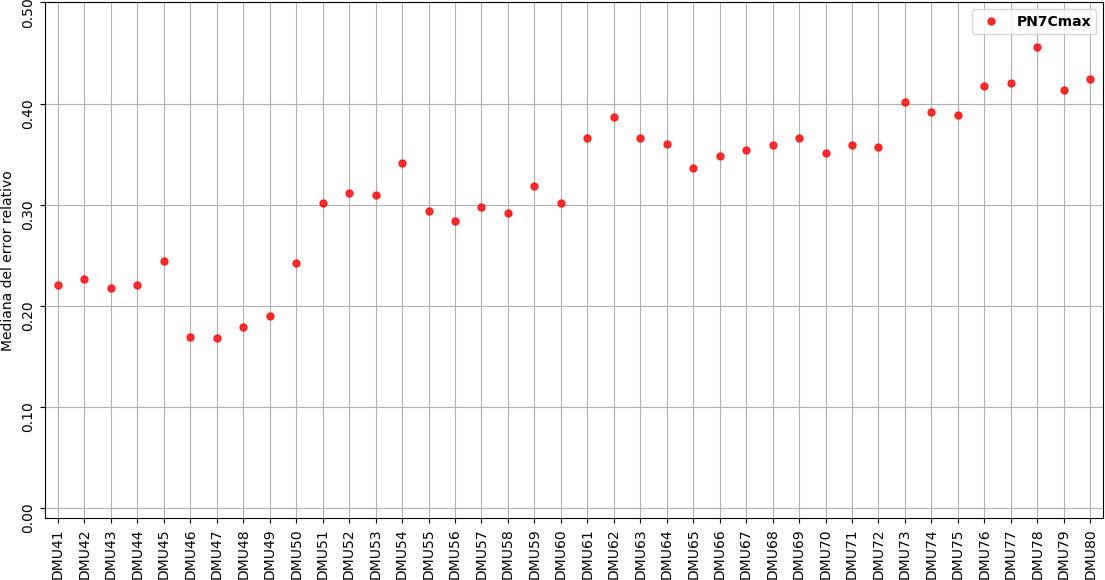
\includegraphics[scale=.65]{Imagenes/resn7ils2.png}
        \caption{Resultados para las instancias \textbf{DMU41-80}}
    \end{subfigure}
    \caption{Resultados para la propuesta más simple. Se marcan los casos en los que se llegó a la mejor solución conocida.}
\end{figure}

Podemos observar que la mediana del error relativo para la segunda mitad de las instancias es considerablemente mayor que para la primera mitad. Estos resultados sirven como un punto de comparación para todas modificaciones.

\section{Función de fitness}
  La función de fitness se obtiene al construir la dupla formada por el makespan y la característica en ese orden. Para determinar cuál es la que obtiene mejores resultados las modificaciones se comparan a pares en cada instancia. Si se encuentra que la diferencia entre dos modificaciones es estadísticamente significativa, se le suma un punto a la ganadora y se le resta uno a la perdedora.
Para determinar si los conjuntos de resultados muestran diferencias estadísticamente significativas se utiliza la prueba de Wilcoxon con un nivel de significancia de $0.01$. 

Los resultados para las propuestas mostradas en \ref{prop:fitness} pueden verse de manera condensada en la siguiente figura. El cuadro $(i,j)$ muestra el número de veces que $i$ fue mejor que $j$.\\
Todas las pruebas se realizaron con la vecindad N7. Se muestra también una tupla construida con las características que obtuvieron mejores resultados. Estas características se ordenan de acuerdo a su número de comparaciones ganadas totales.
\begin{figure}[H]
    \centering
    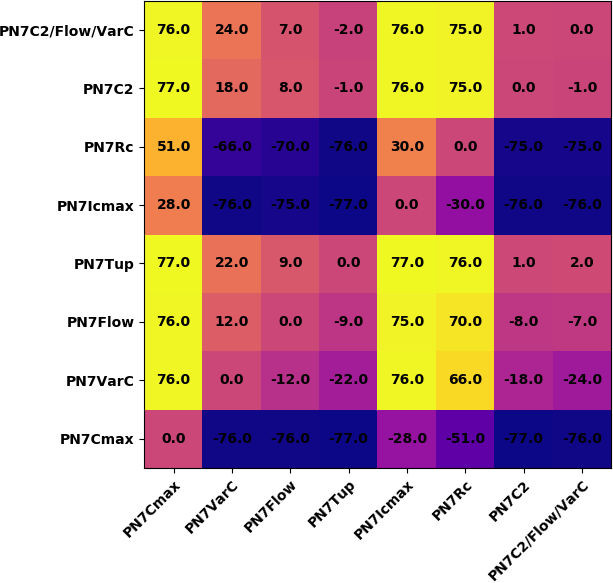
\includegraphics[scale=.8]{Imagenes/fitnesscomp.png}
    \caption{Condensado de los resultados para las modificaciones a la función de fitness. }
\end{figure}

Los mejores resultados se obtienen al construir la tupla mencionada previamente por lo que de ahora en adelante la función de fitness queda fija de esta manera y en los resultados subsecuentes solo se considera este caso. Los resultados detallados se muestran en el apéndice \ref{app:resn7tuple}.

\section{Extensión a vecindad N7}
Los resultados para la extensión que considera movimientos con espacios de inactividad de las máquinas se comparan con los mejores mostrados en la sección pasada. Se sigue el mismo procedimiento que en la sección anterior para hacer esta comparación.

\begin{figure}[H]
    \centering
    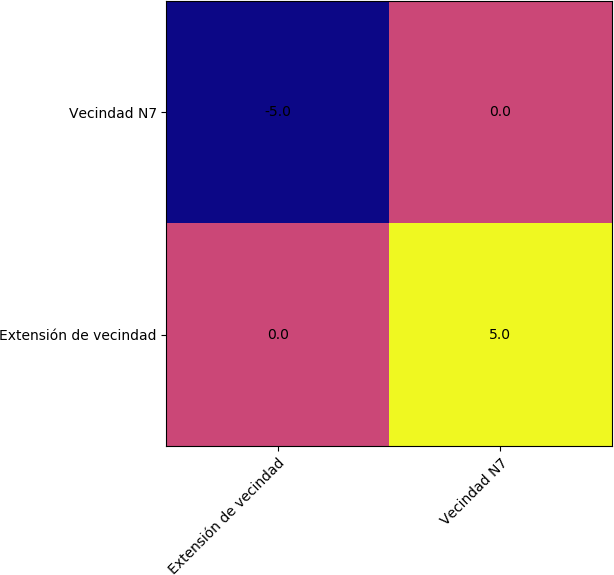
\includegraphics[scale=.7]{Imagenes/n8vsn7.png}
    \caption{Resultados de la comparación}
\end{figure}

También se muestra de manera gráfica los resultados para todas las instancias junto con los mejores resultados de la sección anterior. Los resultados detallados para la extensión propuesta se encuentran en el apéndice \ref{app:resn8tuple}.

\begin{figure}[H]
    \begin{subfigure}{\textwidth}
        \centering
        %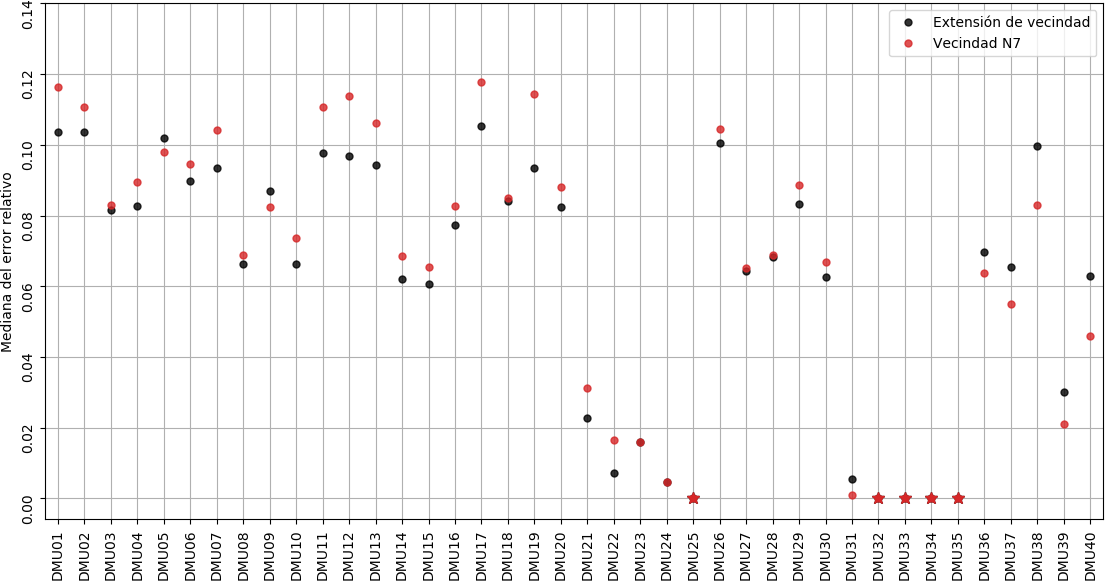
\includegraphics[height=.78\textwidth,width=.95\textheight,angle=270]{Imagenes/n8vsn7err1.png}
        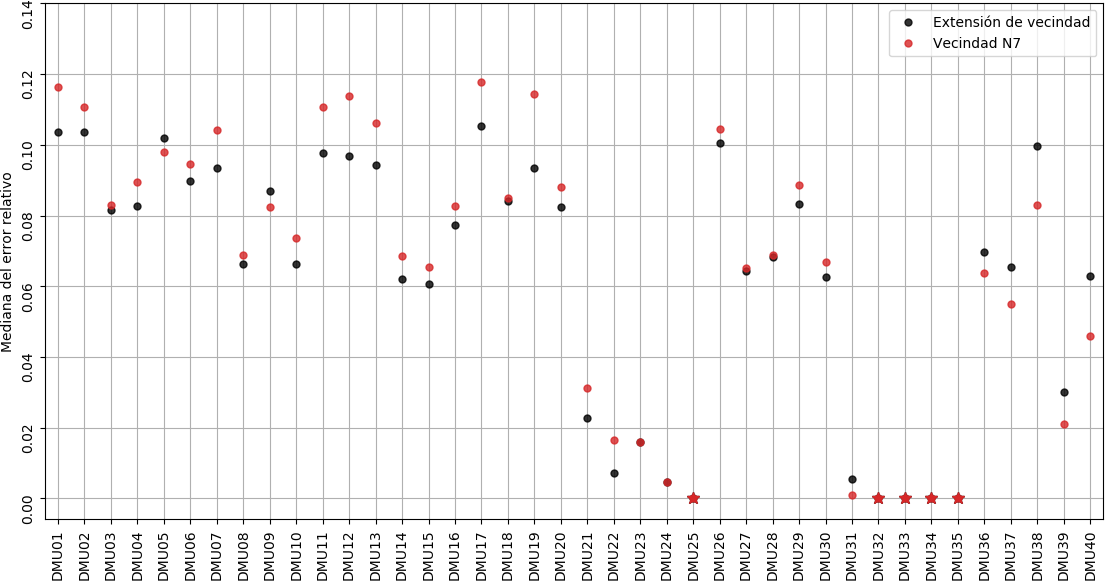
\includegraphics[scale=.6]{Imagenes/n8vsn7err1.png}
        \caption{Resultados para las instancias \textbf{DMU01-40}}
    \end{subfigure}
\end{figure}
\begin{figure}[H]\ContinuedFloat
    \begin{subfigure}{\textwidth}
        \centering
        %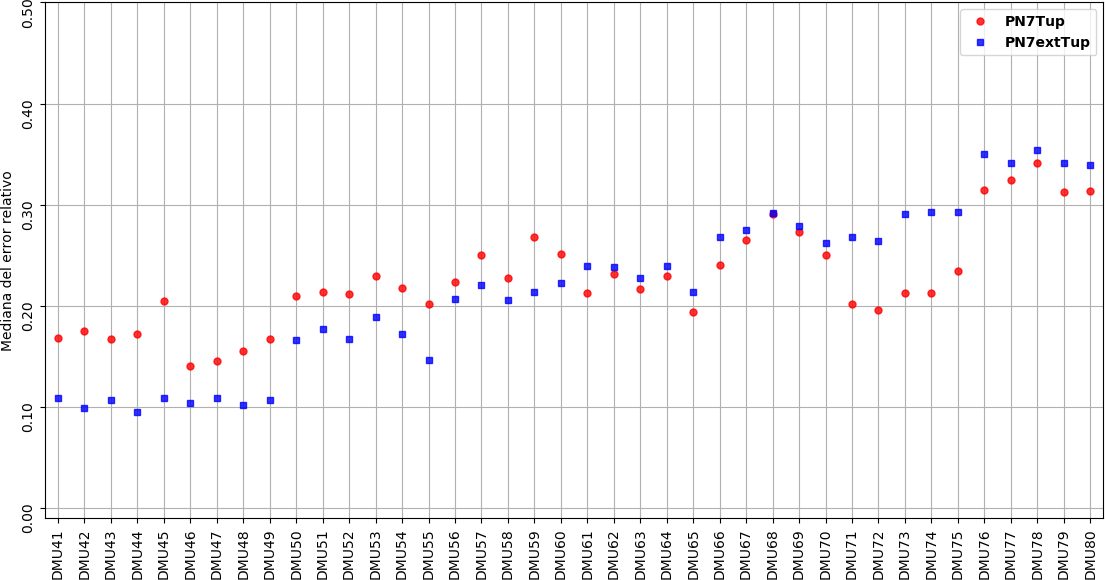
\includegraphics[height=.78\textwidth,width=.95\textheight,angle=270]{Imagenes/n8vsn7err2.png}
        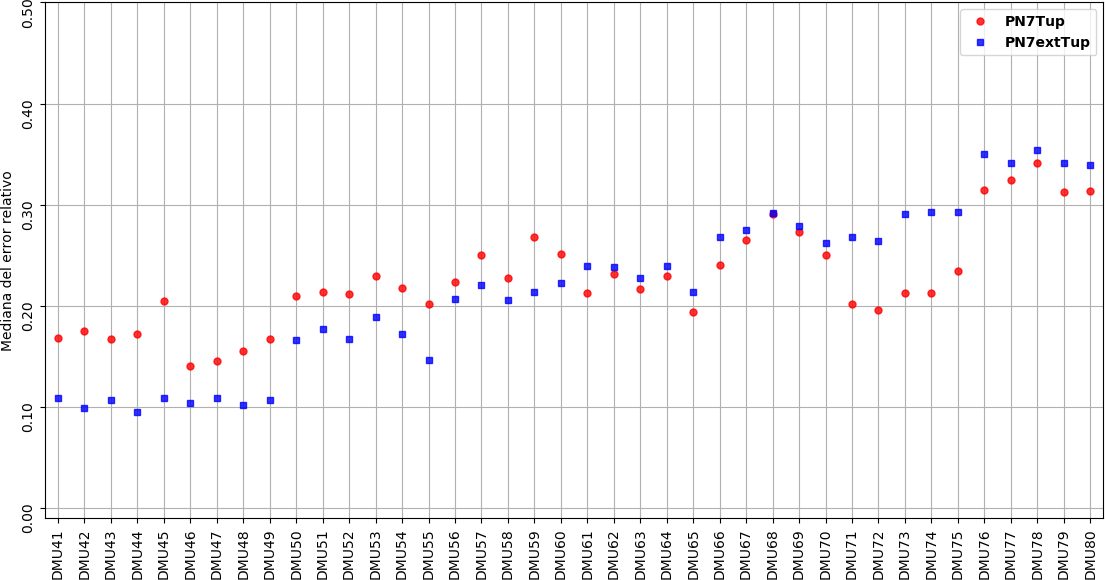
\includegraphics[scale=.6]{Imagenes/n8vsn7err2.png}
        \caption{Resultados para las instancias \textbf{DMU41-80}}
    \end{subfigure}
    \caption{Resultados para ambos métodos. Se marcan los casos en los que se llegó a la mejor solución conocida.}
\end{figure}

\section{Cambio de representación y vecindad}
El cambio de representación y vecindad se compara con las dos propuestas previas. Se sigue el mismo procedimiento mencionado para determinar si hay una diferencia significativa entre los resultados obtenidos.
\begin{figure}[H]
    \centering
    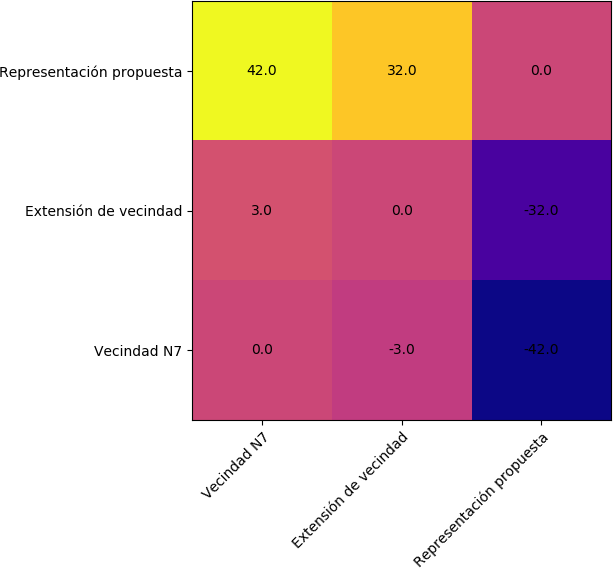
\includegraphics[scale=.7]{Imagenes/prn7n8comp.png}
    \caption{Resultados de la comparación entre los tres métodos.}
\end{figure}
También se muestra la mediana del error relativo alcanzado por los distintos métodos. Los resultados detallados para la extensión de vecindad se encuentran en el apéndice \ref{app:resprtuple}.

\begin{figure}[H]
    \begin{subfigure}{\textwidth}
        \centering
        %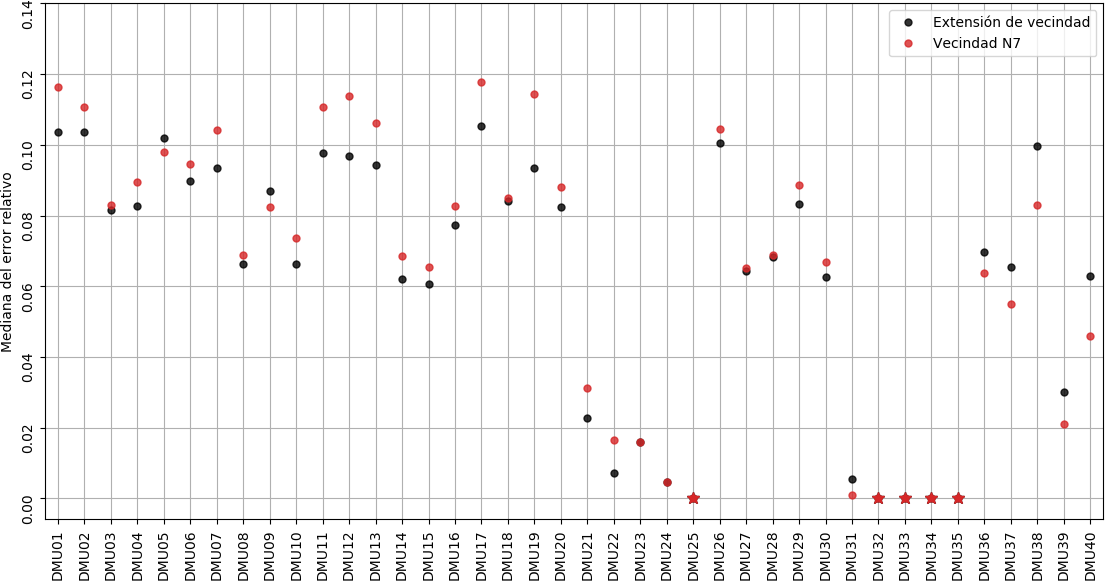
\includegraphics[height=.78\textwidth,width=.95\textheight,angle=270]{Imagenes/n8vsn7err1.png}
        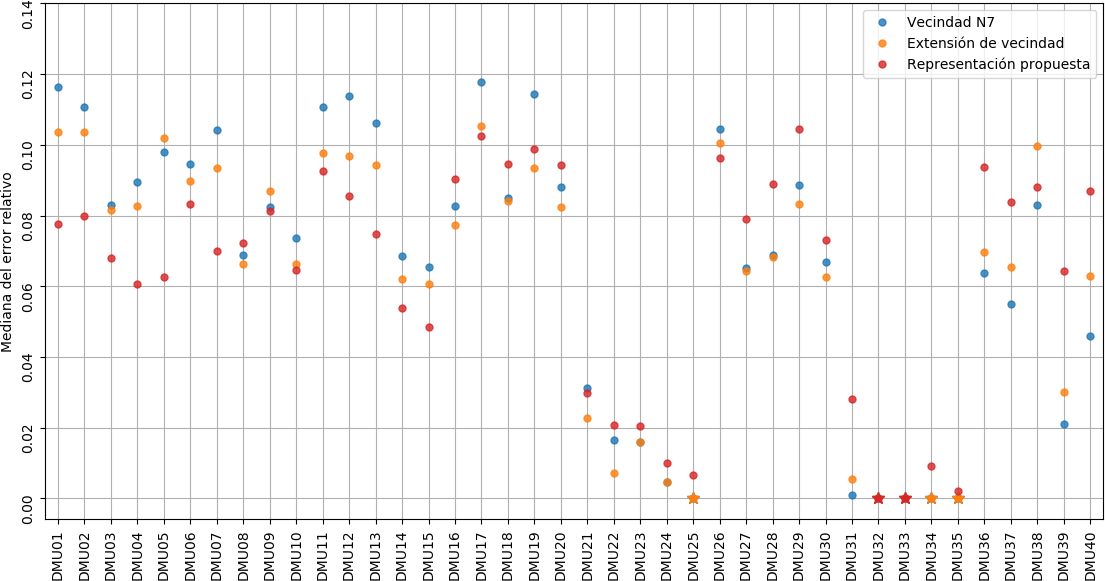
\includegraphics[scale=.6]{Imagenes/prvsn7vsn8err1.png}
        \caption{Resultados para las instancias \textbf{DMU01-40}}
    \end{subfigure}
\end{figure}
\begin{figure}[H]\ContinuedFloat
    \begin{subfigure}{\textwidth}
        \centering
        %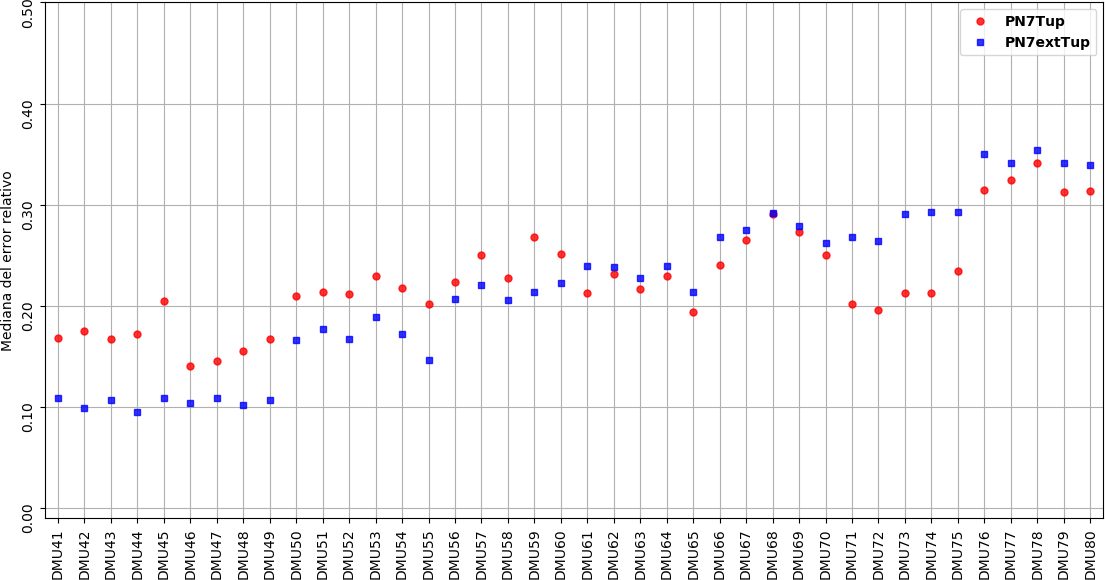
\includegraphics[height=.78\textwidth,width=.95\textheight,angle=270]{Imagenes/n8vsn7err2.png}
        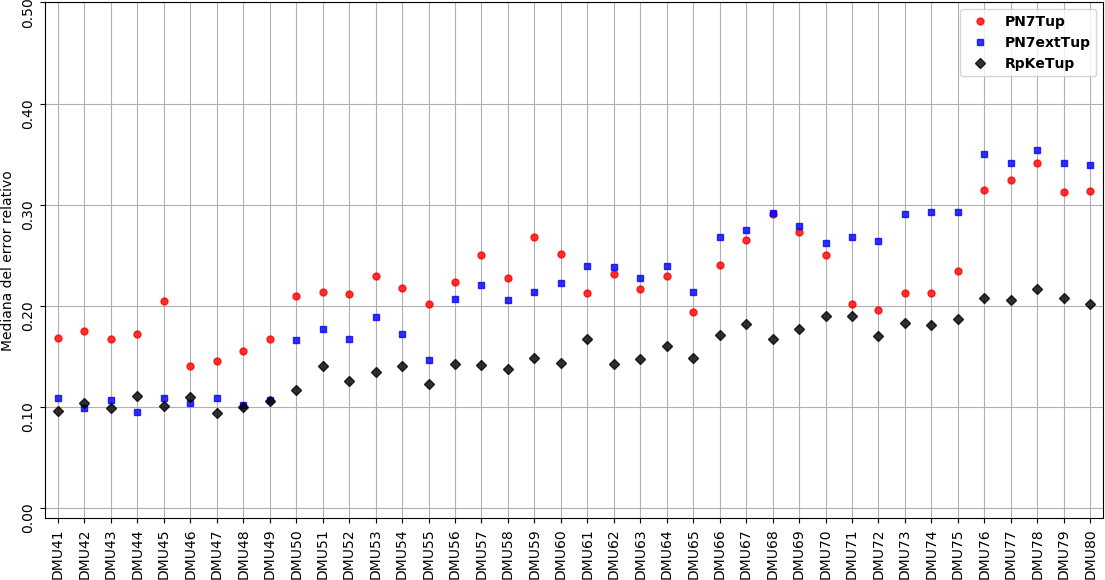
\includegraphics[scale=.6]{Imagenes/prvsn7vsn8err2.png}
        \caption{Resultados para las instancias \textbf{DMU41-80}}
    \end{subfigure}
    \caption{Resultados para ambos métodos. Se marcan los casos en los que se llegó a la mejor solución conocida.}
\end{figure}


Para resaltar las diferencias entre los dos métodos se tomó la instancia en la que se obtuvieron los resultados más dispares, en este caso fue la \textbf{DMU78} y se registró para cada óptimo local visitado su makespan así como el tamaño de su vecindad.

\begin{figure}[H]
    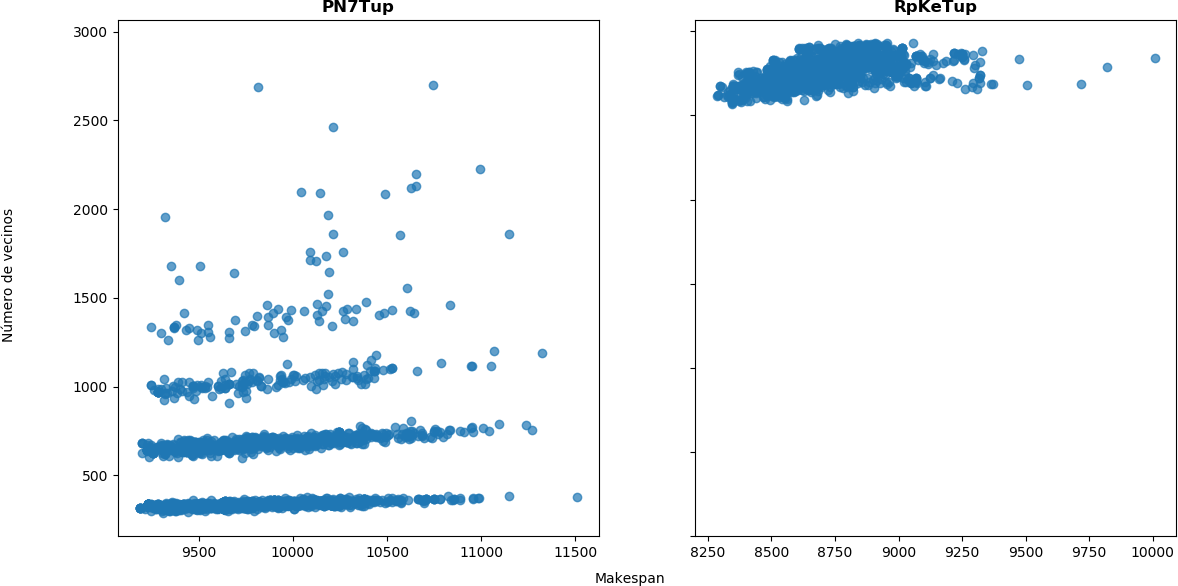
\includegraphics[scale=.6]{Imagenes/compvec78.png}
    \caption{Comparación de tamaño de la vecindad contra makespan de los óptimos locales para la instancia \textbf{DMU78} }
    \label{fig:mattgraph}
\end{figure}

Otro modo de visualizar las diferencias entre ambas representaciones también se presentan diagramas de caja para la diferencia relativa relativa del makespan de los óptimos locales con sus vecinos. Esto nos da una idea de cómo se relacionan las soluciones de acuerdo con su makespan. Si estos valores son muy cercanos entre sí esto nos da un indicio de la suavidad del paisaje de búsqueda.
\begin{figure}[H]
    \begin{subfigure}{\textwidth}
        \centering
        %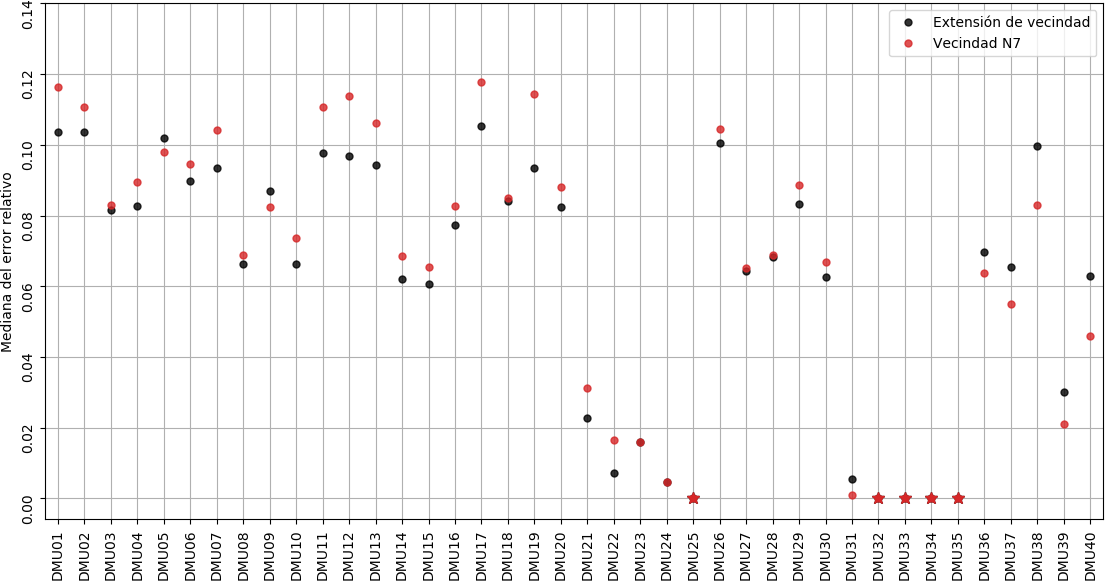
\includegraphics[height=.78\textwidth,width=.95\textheight,angle=270]{Imagenes/n8vsn7err1.png}
        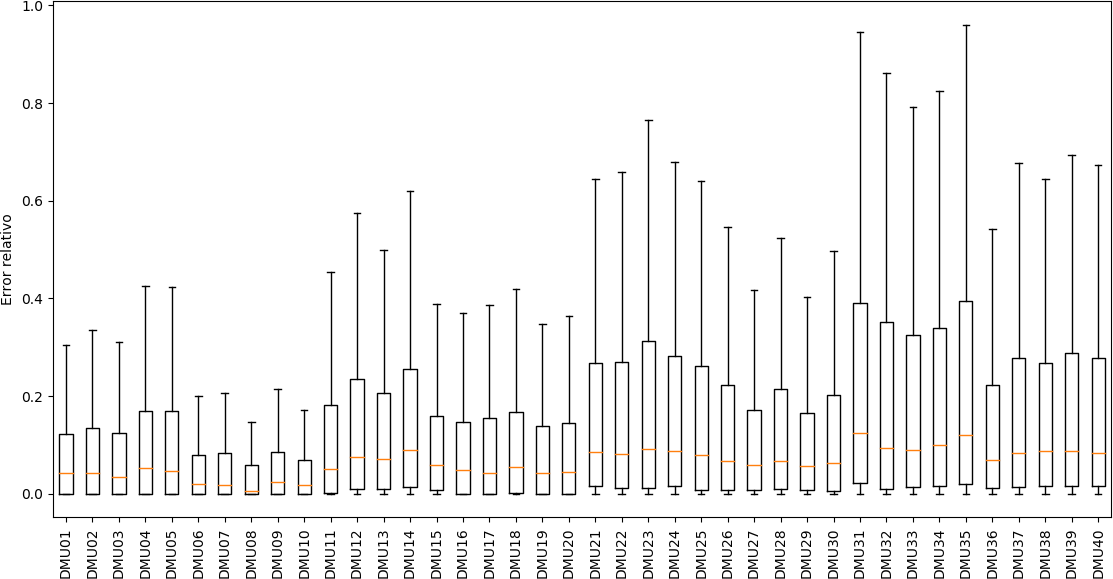
\includegraphics[scale=.6]{Imagenes/bxpn7_1.png}
        \caption{Representación original con vecindad n7 instancias \textbf{DMU01-40}}
    \end{subfigure}
\end{figure}
\begin{figure}[H]\ContinuedFloat
    \begin{subfigure}{\textwidth}
        \centering
        %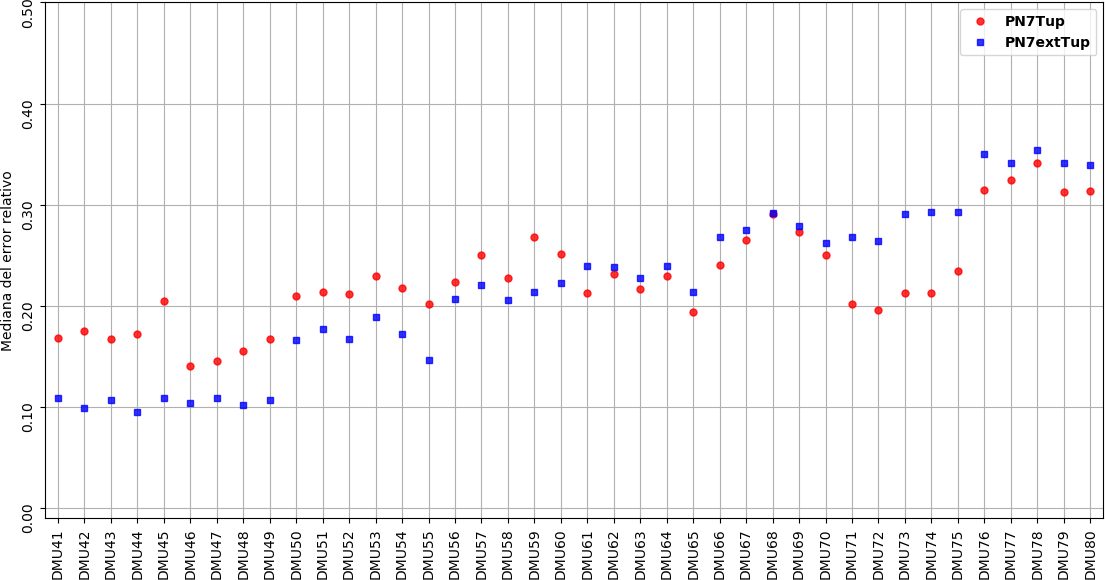
\includegraphics[height=.78\textwidth,width=.95\textheight,angle=270]{Imagenes/n8vsn7err2.png}
        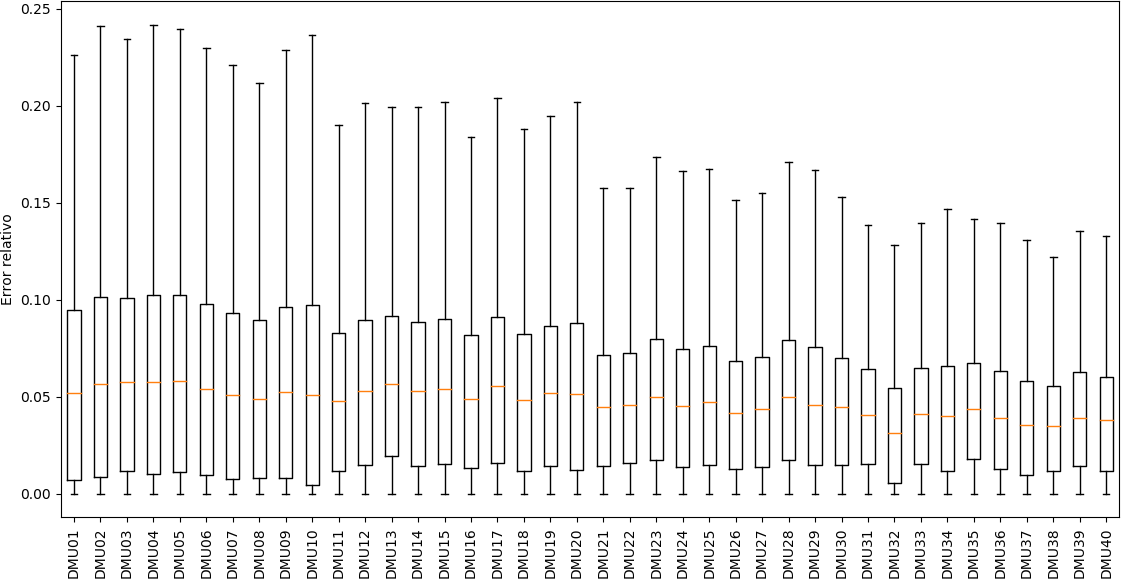
\includegraphics[scale=.6]{Imagenes/bxppr_1.png}
        \caption{Representación propuesta instancias \textbf{DMU01-40}}
    \end{subfigure}
    \caption{Diagramas de caja de la diferencia relativa en makespan de un óptimo local con sus vecinos}
    \label{fig:bxp1}
\end{figure}

\begin{figure}[H]
    \begin{subfigure}{\textwidth}
        \centering
        %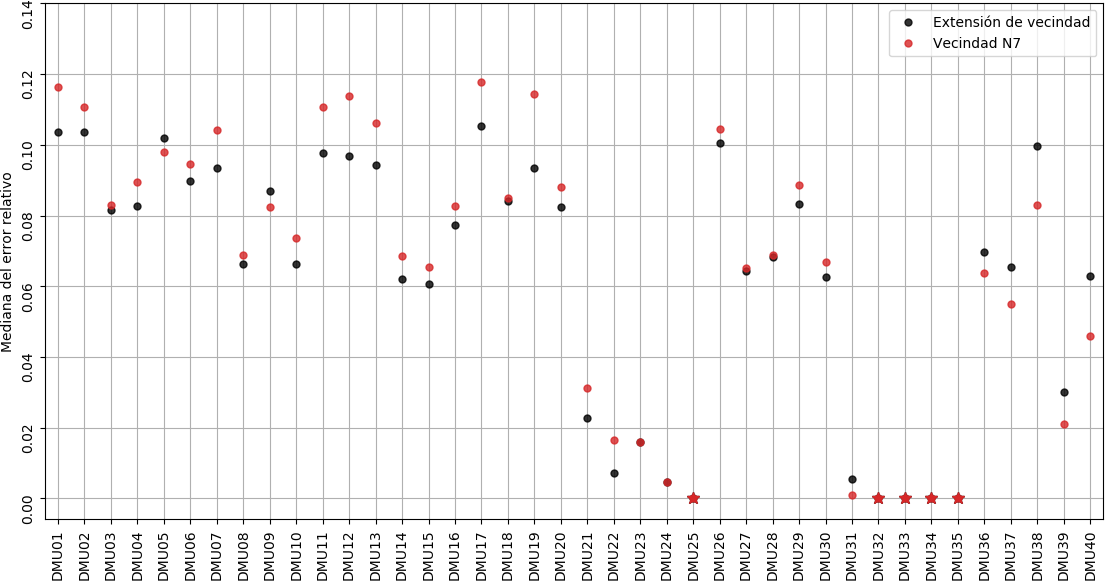
\includegraphics[height=.78\textwidth,width=.95\textheight,angle=270]{Imagenes/n8vsn7err1.png}
        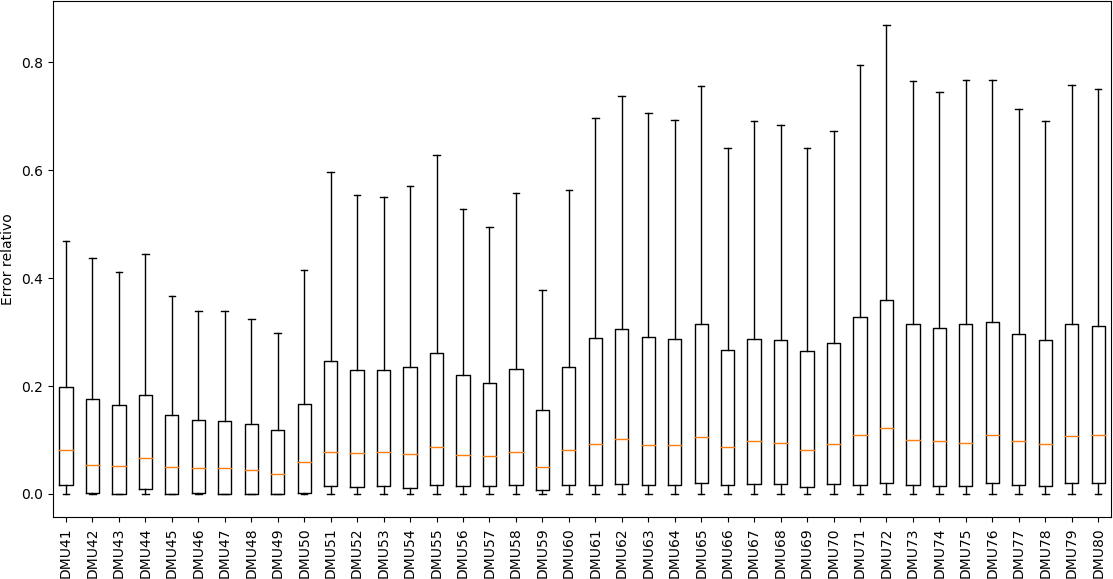
\includegraphics[scale=.6]{Imagenes/bxpn7_2.png}
        \caption{Representación original con vecindad n7 instancias \textbf{DMU41-80}}
    \end{subfigure}
\end{figure}
\begin{figure}[H]\ContinuedFloat
    \begin{subfigure}{\textwidth}
        \centering
        %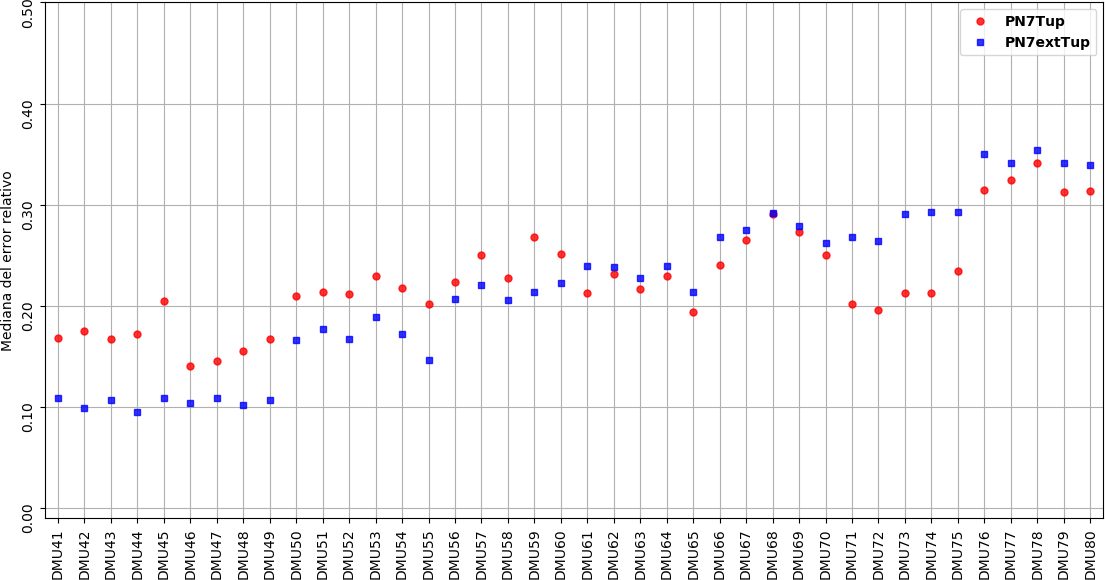
\includegraphics[height=.78\textwidth,width=.95\textheight,angle=270]{Imagenes/n8vsn7err2.png}
        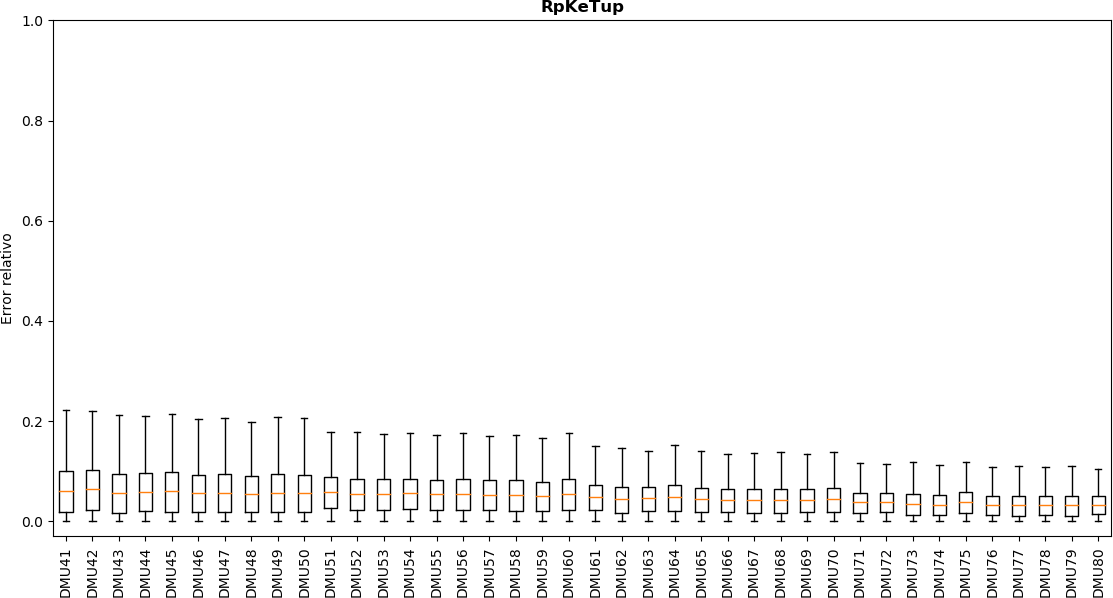
\includegraphics[scale=.6]{Imagenes/bxppr_2.png}
        \caption{Representación propuesta instancias \textbf{DMU41-80}}
    \end{subfigure}
    \caption{Diagramas de caja de la diferencia relativa en makespan de un óptimo local con sus vecinos}
    \label{fig:bxp2}
\end{figure}

En las figuras \ref{fig:bxp1} y \ref{fig:bxp2} observamos que los vecinos de los óptimos locales para la nueva representación y vecindad son más parecidos.

% resultados


%Conclusiones 
\newpage
\chapter{Conclusiones y Trabajos a Futuro}\label{cap:ct} \minitoc
\section{Conclusiones}
Los resultados obtenidos muestran una clara diferencia entre las instancias \textbf{DMU01-40} y las \textbf{DMU41-80} en cuestión de dificultad. 

La búsqueda local iterada con la vecindad N7 y la función de fitness propuesta muestra un desempeño muy diferente en las dos mitades. En la primera mitad se obtienen resultados con bajo error relativo e inclusive en varias ocasiones se alcanzan los resultados del estado del arte mientras que en la segunda mitad el error relativo es bastante más alto y se crece con el tamaño de la instancia considerada. 
La extensión propuesta no mostró ventajas importantes frente a la vecindad N7 y muestra el mismo comportamiento a pesar de plantearse como una posible manera de escapar de óptimos locales. 

La función de fitness planteada en general muestra que es benéfico considerar características de la planificación a demás del makespan para obtener mejores resultados. Aunque sí se tienen mejoras con la adición de estas características es posible que exista una mejor manera de construir la función de fitness para lograr una mejor exploración del pasaje de búsqueda.

El cambio de representación tuvo en gran efecto en la mejora del desempeño de la búsqueda local. Este cambio logra una disminución sustancial del error relativo en la segunda mitad de las instancias. Puede observarse en la figura \ref{fig:mattgraph} que en esta nueva estructura de vecindad el tamaño de la misma está mucho más relacionado con el makespan de la solución. También puede verse que el cambio de representación desde un inicio restringe a soluciones de mucha más calidad y que están más conectadas que las que se encuentran con la vecindad N7. 





\appendix
\appendix


 \newpage

\bibliographystyle{acm}
\bibliography{Referencias}

\end{document}
